%%%%%%%%%%%%%%%%%%%%%%%%%%%%%%%%%%%%%%%%%
% Beamer Presentation
% LaTeX Template
% Version 1.0 (10/11/12)
%
% This template has been downloaded from:
% http://www.LaTeXTemplates.com
%
% License:
% CC BY-NC-SA 3.0 (http://creativecommons.org/licenses/by-nc-sa/3.0/)
%
%%%%%%%%%%%%%%%%%%%%%%%%%%%%%%%%%%%%%%%%%

%----------------------------------------------------------------------------------------
%	PACKAGES AND THEMES
%----------------------------------------------------------------------------------------

\documentclass{beamer}
\usepackage{xeCJK}
\usepackage{times}
\usepackage{multirow}
\usepackage{diagbox}
\usepackage{subfigure}
\usepackage{graphicx}
\usepackage{booktabs}
\usepackage{float}
\usepackage{algorithm}
\usepackage{algorithmic}
%\usepackage{caption}

\floatname{algorithm}{算法}  
\renewcommand{\algorithmicrequire}{\textbf{初始化:}}  
\renewcommand{\algorithmicensure}{\textbf{直到收敛,返回}}
%\renewcommand{\algorithmicrepeat}{\textbf{迭代,根据以下步骤更新:}}
\newcommand{\INDSTATE}[1][1]{\STATE\hspace{#1\algorithmicindent}}
\DeclareMathOperator*{\argmax}{arg\,max}
%\captionsetup[subfigure]{labelformat=empty}
\setbeamertemplate{caption}[numbered]

\newcommand{\cccve}{CCC\{$v_\mathrm{e}$\}}
\newcommand{\ccckt}{CCC\{$K^\mathrm{trans}$\}}
\newcommand{\kt}{$K^\mathrm{trans}$}
\newcommand{\Ve}{$v_\mathrm{e}$}
\newcommand{\argmin}{\operatornamewithlimits{arg\ min~}}

%\setCJKfamilyfont{song}{SimSun}                             %宋体 song
%\newcommand{\song}{\CJKfamily{song}} 

\usefonttheme{serif}
\usepackage{fourier}
\mode<presentation> {

% The Beamer class comes with a number of default slide themes
% which change the colors and layouts of slides. Below this is a list
% of all the themes, uncomment each in turn to see what they look like.

%\usetheme{default}
%\usetheme{AnnArbor}
%\usetheme{Antibes}
%\usetheme{Bergen}
%\usetheme{Berkeley}
%\usetheme{Berlin}
%\usetheme{Boadilla}
%\usetheme{CambridgeUS}
%\usetheme{Copenhagen}
%\usetheme{Darmstadt}
%\usetheme{Dresden}
%\usetheme{Frankfurt}
%\usetheme{Goettingen}
%\usetheme{Hannover}
%\usetheme{Ilmenau}
%\usetheme{JuanLesPins}
%\usetheme{Luebeck}
%\usetheme{Madrid}
\usetheme{Malmoe}
%\usetheme{Marburg}
%\usetheme{Montpellier}
%\usetheme{PaloAlto}
%\usetheme{Pittsburgh}
%\usetheme{Rochester}
%\usetheme{Singapore}
%\usetheme{Szeged}
%\usetheme{Warsaw}

% As well as themes, the Beamer class has a number of color themes
% for any slide theme. Uncomment each of these in turn to see how it
% changes the colors of your current slide theme.

%\usecolortheme{albatross}
%\usecolortheme{beaver}
%\usecolortheme{beetle}
%\usecolortheme{crane}
%\usecolortheme{dolphin}
%\usecolortheme{dove}
%\usecolortheme{fly}
%\usecolortheme{lily}
%\usecolortheme{orchid}
%\usecolortheme{rose}
%\usecolortheme{seagull}
%\usecolortheme{seahorse}
%\usecolortheme{whale}
%\usecolortheme{wolverine}

%\setbeamertemplate{footline} % To remove the footer line in all slides uncomment this line
%\setbeamertemplate{footline}[page number] % To replace the footer line in all slides with a simple slide count uncomment this line

%\setbeamertemplate{navigation symbols}{} % To remove the navigation symbols from the bottom of all slides uncomment this line
}

%\usepackage{graphicx} % Allows including images
 % Allows the use of \toprule, \midrule and \bottomrule in tables

%----------------------------------------------------------------------------------------
%	TITLE PAGE
%----------------------------------------------------------------------------------------

\title[博士学位论文答辩]{基于变分和稀疏表示的定量MR图像\\快速重建模型和加速算法}

\author[南京理工大学]{
答辩人:王冬 \\
导师:杨孝平\quad 教授
} % Your name
\institute[南京理工大学] % Your institution as it will appear on the bottom of every slide, may be shorthand to save space
{
南京理工大学 \\ % Your institution for the title page
\medskip
理学院 
}
\date{2020年01月04日} % Date, can be changed to a custom date

\begin{document}

\begin{frame}
\titlepage % Print the title page as the first slide
\end{frame}

%----------------------------------------------------------------------------------------
%	PRESENTATION SLIDES
%----------------------------------------------------------------------------------------

%------------------------------------------------
\section{引言}
%------------------------------------------------
%\AtBeginSection[]
%{
    \begin{frame}
        \tableofcontents[currentsection,hideallsubsections]
    \end{frame}
%}

\subsection{研究背景}
\begin{frame}
%\frametitle{研究背景——核磁共振成像}
核磁共振成像(MRI),尤其是动态MRI和定量MRI是医学临床和研究中常用的成像方式。
\begin{figure}[htbp]
\begin{minipage}[t]{0.35\textwidth}
\centering
\includegraphics[width=\textwidth]{../img/intro/breast.png}
\\ 磁共振动态造影增强
\end{minipage}
\hfill
\begin{minipage}[t]{0.165\textwidth}
\centering
\includegraphics[width=\textwidth]{../img/intro/perfusion.png}
\\心脏灌注
\end{minipage}
\hfill
\begin{minipage}[t]{0.35\textwidth}
\centering
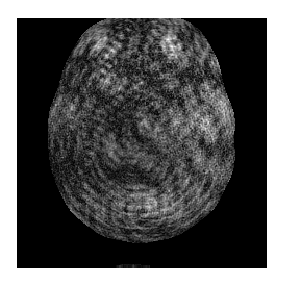
\includegraphics
[width=\textwidth]{../img/intro/brain.eps}
\\活体人脑磁共振指纹
\end{minipage}
\end{figure}
\end{frame}

\begin{frame}
	\frametitle{动态MR成像的数学模型}
%		\item 动态MR成像过程通常被建模为Fourier编码,即首先从图像的Fourier域(通常称为kt-space)中采样,再通过算法将图像重建出来。
记动态MR图像为$X\in \mathbb{C}^{N_1\times N_2\times d}$,则动态MR成像的过程相当于在噪声的干扰下,在Fourier域中(也称为kt-space)进行采样
\begin{equation}
	B=AX+\epsilon,
\end{equation}
其中$A=\mathcal{M}\cdot\mathcal{F}$是采样算子,$\mathcal{F}$是作用在每一帧图像上的二维Fourier变换,$\mathcal{M}$是作用在每一帧图像上的二维采样模式,$\epsilon$是加性高斯白噪声。
\vspace{1cm}\\
\large{\textbf{问题:成像速度慢!}}
\end{frame}

\begin{frame}
	\frametitle{基于压缩感知的快速MR成像}
	\begin{itemize}
		\item 压缩感知理论是由Candès等提出的采样理论,是目前快速MR成像的主流方法。
		\item 假设图像在某个变换域\textbf{稀疏}的前提下,对图像进行\textbf{非相干下采样},通过\textbf{非线性重建}算法可以高概率地将图像重建出来。
	\end{itemize}

基于压缩感知的动态MR图像重建模型为:
	\begin{equation}
	\min_X \frac{1}{2}\|AX-B\|_{\mathrm{F}}^2+\alpha\|\Phi X\|_1,
	\end{equation}
其中$\Phi$是某个稀疏变换,$\alpha>0$是平衡数据项和稀疏正则项的参数,$\mathrm{F}$为Frobenius范数。这里$A$为下采样算子。

%这里$A\in \mathbb{C}^{M_1\times M_2\times d}$为下采样算子,且$M_1M_2<<N_1N_2$.
\end{frame}

\begin{frame}
%	\frametitle{已有的模型和方法}
	\begin{itemize}
		\item 常用的稀疏表示:Fourier变换、小波变换、多尺度分析、全变差(TV)、广义全变差(TGV)、核范数、字典学习、深度神经网络等
		\item 常用的采样方式:Cartesian采样、伪径向/径向采样、螺旋采样等
		\item 常用的重建算法:ADMM、FISTA、Primal-Dual等
	\end{itemize}
\begin{figure}[htbp]
\begin{minipage}[t]{0.3\textwidth}
\centering
\includegraphics[width=\textwidth]{../img/intro/cartesian.png}
\\ Cartesian采样
\end{minipage}
\hfill
\begin{minipage}[t]{0.3\textwidth}
\centering
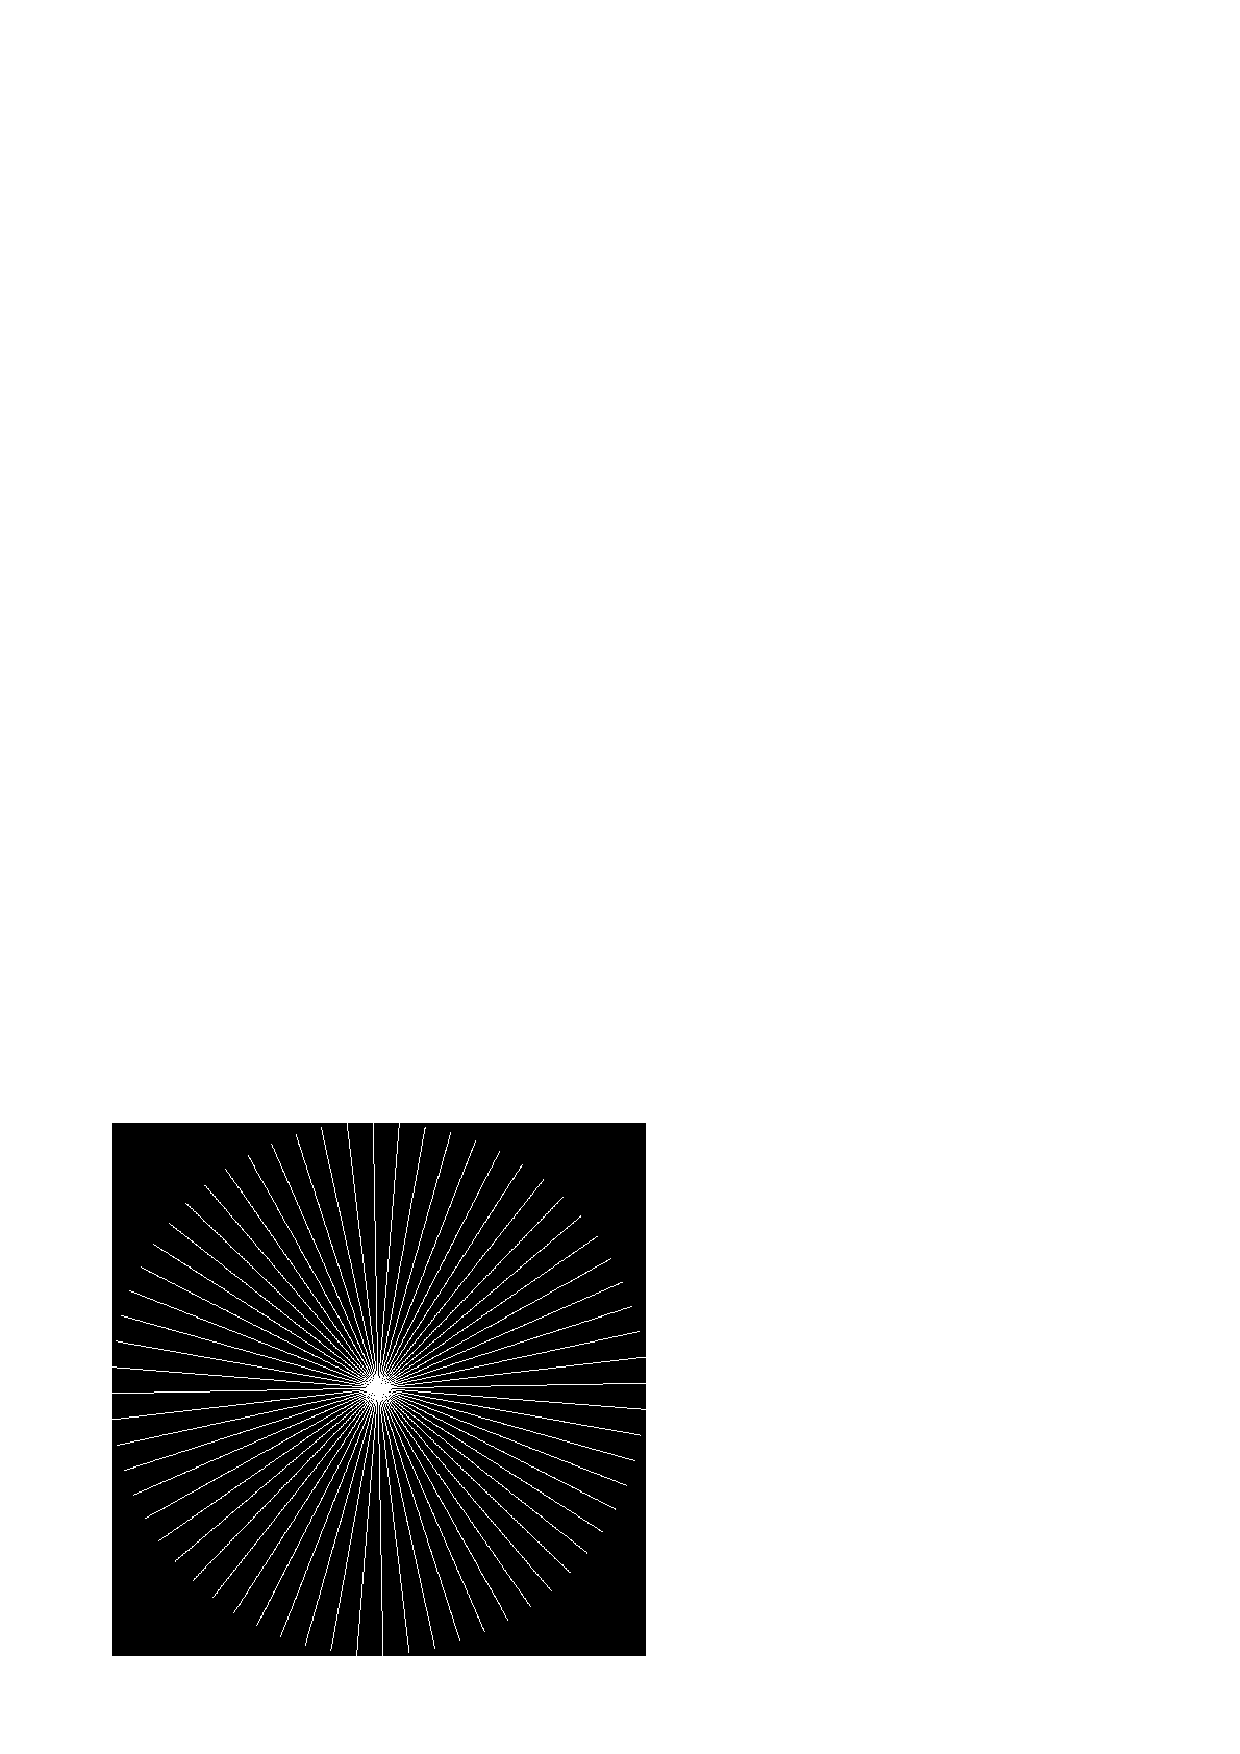
\includegraphics[width=\textwidth]{../img/intro/radial.png}
\\径向采样
\end{minipage}
\hfill
\begin{minipage}[t]{0.3\textwidth}
\centering
\includegraphics
[width=\textwidth]{../img/intro/spiral.png}
\\螺旋采样
\end{minipage}
\end{figure}
\end{frame}


%\begin{frame}
%	\frametitle{动态MR重建中存在的问题}
%%	动态MR重建中存在的问题:
%	\begin{itemize}
%		\item 重建速度慢,如磁共振动态对比增强(DCE-MRI)、磁共振指纹成像(MRF)中字典生成与参数图的重建等
%		\item 现有的动态MR图像重建模型存在空间伪影严重、边缘不清等问题,尤其在胸部DCE-MRI图像上
%		\item 对于胸部DCE-MRI,其适用的时间方向上的稀疏正则项是未知的
%	\end{itemize}
%\end{frame}

%------------------------------------------------
\subsection{论文研究动机和研究成果}
\begin{frame}
\textbf{研究动机:}
	\begin{itemize}
		\item 重建速度慢,如磁共振动态对比增强(DCE-MRI)、磁共振指纹成像(MRF)中字典生成与参数图的重建等
		\item 现有的动态MR图像重建模型存在空间伪影严重、边缘不清、像素时间曲线拟合差等问题,尤其在胸部DCE-MRI图像上
		\item 临床上适用于胸部DCE-MRI的时间方向上的稀疏表示是未知的
	\end{itemize}
	\textbf{研究成果:}
	\begin{itemize}
		\item 针对动态MR图像,结合压缩感知和图像分解的思想,提出了基于二阶时空TGV和核范数的重建模型
		\item 通过定量分析的方式比较和评估了五种不同的时间方向的稀疏变换,确定了适用于胸部DCE-MRI的时间稀疏正则项
		\item 利用图形处理单元(GPU)加速MRF字典生成与匹配,并设计开发了一款基于CUDA框架的开源程序snapMRF
	\end{itemize}
\end{frame}

%------------------------------------------------
\section{动态MR图像的低秩和稀疏分解的高阶变分模型和算法}
%------------------------------------------------
%\AtBeginSection[]
%{
    \begin{frame}
        \tableofcontents[currentsection,hideallsubsections]
    \end{frame}
%}

\subsection{低秩和稀疏分解模型}
%\begin{frame}
%	\frametitle{基于压缩感知的动态MR图像重建模型}
%	目前基于压缩感知模型的动态MR图像重建有以下三个策略:
%	\begin{itemize}
%		\item 仅利用动态MR图像的稀疏性		
%	\end{itemize}
%	k-t SPARSE:
%	\begin{equation}
%	\min_X\frac{1}{2}||AX-B||_{\mathrm{F}}^2 + \alpha||\mathcal{W}X||_1 + \beta||\mathcal{F}_tX||_1,
%	\end{equation}
%	其中$\mathcal{W}$是空间方向上的二维小波变换,而$\mathcal{F}_t$是时间上的一维Fourier变换。
%	
%	问题:胸部DCE-MRI图像通常不会表现出周期性。	
%\end{frame}
%
%\begin{frame}
%	\frametitle{基于压缩感知的动态MR图像重建模型}
%	\begin{itemize}
%		\item 考虑动态MR图像的低秩性,找到一个既稀疏又低秩的解		
%	\end{itemize}
%	k-t SLR:
%	\begin{equation}
%		\min_X \frac{1}{2}\|AX-B\|_{\mathrm{F}}^2+\alpha\mathrm{TV}(X)+\beta\|X\|_1.
%	\end{equation}
%	这里
%$$\mathrm{TV}(\cdot)=\|\nabla_3\cdot\|_1,\quad |\nabla_3\cdot| = \sqrt{(\nabla_x\cdot)^2+(\nabla_y\cdot)^2+\mu(\nabla_t\cdot)^2},$$
%其中$\nabla_x$,$\nabla_y$和$\nabla_t$分别为$x$,$y$和$t$方向上的梯度算子,$\mu$是平衡空间稀疏性与时间稀疏性的参数。
%
%问题:算法重建速度慢,重建图像中易出现阶梯效应
%\end{frame}

\begin{frame}
	\frametitle{动态MR图像重建的低秩和稀疏分解模型}
	\textbf{图像分解模型}是将动态MR图像建模为稀疏部分和低秩部分的加和,并分别用不同的正则项来约束:
    \begin{equation}
    	\min_{L,S}\frac{1}{2}||A(L+S)-B||_\mathrm{F}^2 + \alpha||\Phi S||_1 + \beta\|L\|_*,
    \end{equation}
     其中$L$和$S$分别为低秩部分和稀疏部分,$\|\cdot\|_*$为核范数,即矩阵奇异值的和。
     
     \textbf{$\Phi$的选择:}
     \begin{itemize}
     	\item 时间方向的一维Fourier变换($\mathcal{F}_t$)$\Rightarrow$ 仅适用于具有周期性的图像
     	\item 时间方向的梯度算子($\nabla_t$)$\Rightarrow$ 仅仅利用了时间方向的稀疏性
     	\item 全变差(TV) $\Rightarrow$ 易产生阶梯效应且计算速度慢
     \end{itemize}
\end{frame}

%\begin{frame}
%	\frametitle{基于压缩感知的动态MR图像重建模型}
%    ICTGV:
%    \begin{equation}
%    	\mathrm{ICTGV}_{\alpha, \beta}^2(X) = \inf_{X=X_1+X_2}\mathrm{TGV}_{\alpha_1}^2(X_1) + \beta\mathrm{TGV}_{\alpha_2}^2(X_2),
%    \end{equation}
%    TGV是经典TV泛函的推广,可以在保持图像边缘的同时有效地抑制阶梯效应。其定义为:
%    $$\mathrm{TGV}_\alpha^2(X)=\min_{\omega\in \mathrm{BD}(w)}\alpha_1\|\nabla_3 X-w\|_1 + \alpha_0\|\mathcal{E}(w)\|_1.$$
%其中$\mathcal{E}(w)=(\nabla_3w+\nabla_3w^{T})/2$是对称梯度算子,$\mathrm{BD}(w)$ 是有界形变函数空间。
%
%    问题:在胸部DCE-MRI图像上的表现是未知的
%\end{frame}

\begin{frame}
\frametitle{二阶时空TGV泛函}
	TGV泛函是经典TV泛函的高阶推广,可以有效地抑制阶梯效应。二阶时空TGV泛函的定义为:
    $$\mathrm{TGV}_\alpha^2(X)=\min_{w\in \mathrm{BD}(\Omega)}\alpha_1\|\nabla_3 X-w\|_1 + \alpha_0\|\mathcal{E}(w)\|_1,$$
其中$\mathcal{E}(w)=(\nabla_3w+\nabla_3w^{T})/2$是对称梯度算子,$\mathrm{BD}(\Omega)$ 是有界形变函数空间。这里
$$|\nabla_3\cdot| = \sqrt{(\nabla_x\cdot)^2+(\nabla_y\cdot)^2+\mu(\nabla_t\cdot)^2},$$
其中$\nabla_x$,$\nabla_y$和$\nabla_t$分别为$x$,$y$和$t$方向上的梯度算子,$\mu>0$是平衡空间与时间的参数。
\end{frame}

\subsection{基于二阶时空TGV和核范数的模型}
\begin{frame}
	\frametitle{基于二阶时空TGV和核范数的模型}
针对动态MR图像,基于图像分解的思想,利用二阶时空TGV和核范数,提出模型:
\begin{equation}
\min_{L,S} \frac{1}{2}\|A(L+S)-B\|_{\mathrm{F}}^2+\mathrm{TGV}^2_\alpha(S)+\beta\|L\|_*.
\label{propopsed}
\end{equation}
\begin{itemize}
	\item 模型是凸的、适定的
	\item 核范数建模时间上高度相关的背景
	\item 二阶时空TGV泛函建模背景之上的动态信息
\end{itemize}
\end{frame}

\begin{frame}
\frametitle{模型的求解}
Primal-Dual算法被广泛地应用到寻找凸-凹鞍点问题的极大极小问题中:
\begin{equation}
\min_{x\in\mathcal{X}}\max_{y\in\mathcal{Y}}\quad\langle \mathcal{K}x,y\rangle+f(x)-g(y).
\label{saddle}
\end{equation}
%其中$\mathcal{X}$和$\mathcal{Y}$是Hilbert空间,$\mathcal{K}:\mathcal{X}\rightarrow\mathcal{Y}$是线性连续映射,并且泛函$f:\mathcal{X}\rightarrow(-\infty,\infty]$和$g:\mathcal{Y}\rightarrow(-\infty,\infty]$是适定的、凸的和下半连续的。
%\begin{equation}
%\min_{x}\max_{y}\quad\langle \mathcal{K}x,y\rangle+f(x)-g(y),
%\label{saddle}
%\end{equation}
Chambolle-Pock迭代格式:
\begin{equation*}
\left\{
\begin{aligned}
&y^{n+1}=(I+\sigma\partial g)^{-1}(y^n+\sigma \mathcal{K}\bar{x}^n), \\
&x^{n+1}=(I+\tau\partial f)^{-1}(x^n-\tau \mathcal{K}^*y^{n+1}), \\
&\bar{x}^{x+1}=2x^{n+1}-x^n.
\end{aligned}
\right.
\end{equation*}
\end{frame}

\begin{frame}
%	\frametitle{模型的离散化}
将模型(\ref{propopsed})进行离散化:
\begin{equation}
\begin{aligned}
	\min_{(S,w,L)\in U\times V\times U} \alpha_1 \|\nabla_3 S-w\|_1&+\alpha_0\|\mathcal{E}(w)\|_1+\beta\|L\|_*\\
	&+\frac{1}{2}\|A(L+S)-B\|_\mathrm{F}^2.
\end{aligned}
\label{discrete}
\end{equation}
相应的鞍点问题为:
\begin{equation}
\begin{aligned}
	\min_{(S,w,L)\in U\times V\times U} &\max_{(p,q,\lambda)\in V\times W\times U} \langle \nabla_3 S-w,p\rangle+\langle\mathcal{E}(w),q\rangle+\beta\|L\|_* \\
	&+\langle A(L+S)-B,\lambda \rangle-\frac{1}{2}\|\lambda\|_\mathrm{F}^2 \\
	&-\mathcal{I}_{\|\cdot\|_\infty\leq\alpha_1}(p)-\mathcal{I}_{\|\cdot\|_\infty\leq\alpha_0}(q).
\end{aligned}
\label{dual}
\end{equation}
%这里$p$,$q$和$\lambda$是对偶变量。
%$V=U\times U\times U$,$W=U\times U\times U\times U\times U\times U$。
\end{frame}

%\begin{frame}
%模型(\ref{discrete})相应的鞍点问题为:
%\begin{equation}
%\begin{aligned}
%	\min_{(S,w,L)\in U\times V\times U} &\max_{(p,q,\lambda)\in V\times W\times Y} \langle \nabla_3 S-w,p\rangle+\langle\mathcal{E}(w),q\rangle+\beta\|L\|_* \\
%	&+\langle A(L+S)-B,\lambda \rangle-\frac{1}{2}\|\lambda\|_\mathrm{F}^2 \\
%	&-\mathcal{I}_{\|\cdot\|_\infty\leq\alpha_1}(p)-\mathcal{I}_{\|\cdot\|_\infty\leq\alpha_0}(q).
%\end{aligned}
%\label{dual}
%\end{equation}
%这里$p$,$q$和$\lambda$是对偶变量,$W=U\times U\times U\times U\times U\times U$。
%\end{frame}

\begin{frame}
%	\frametitle{模型的求解}
	将鞍点问题(\ref{dual})转换为结构(\ref{saddle}),令$$\mathcal{X}=U\times V\times U,\quad \mathcal{Y}=V\times W\times U, \quad
	\mathcal{K}=
\begin{pmatrix}
\nabla_3 & -I & 0\\
0 & \mathcal{E} & 0\\
A & 0 & A
\end{pmatrix},
$$
并且
\begin{equation*}
\begin{aligned}
&f(x)=\beta\|L\|_*,\\
&g(y)=\langle B,\lambda\rangle+\frac{\|\lambda\|_\mathrm{F}^2}{2}+\mathcal{I}_{\|\cdot\|_\infty\leq\alpha_1}(p)+\mathcal{I}_{\|\cdot\|_\infty\leq\alpha_0}(q).
\end{aligned}
\end{equation*}
于是模型(\ref{dual})的求解过程如算法\ref{alg:proposed}的所示。
\end{frame}

\begin{frame}
%	\frametitle{模型的求解}
	\begin{center}
	\scalebox{0.95}{
	\begin{minipage}{1\linewidth}
	\begin{algorithm}[H]
	\caption{二阶时空TGV和低秩分解模型的Primal-Dual算法}
	\label{alg:proposed}
	\begin{algorithmic}
		\REQUIRE $\sigma$, $\tau$, $S_0$, $L_0$,令 $L_0=A^*B$,$S_0=0$;
		\INDSTATE[-1] \textbf{迭代:根据以下步骤更新参数:}	
		\STATE 1. $p^{n+1} = \mathcal{P}_{\alpha_1}(p^n+\sigma(\nabla \bar{S}^n-\bar{w}^n))$;
		\STATE 2. $q^{n+1} = \mathcal{P}_{\alpha_0}(q^n+\sigma\mathcal{E}(\bar{w}^n))$;
		\STATE 3. $\lambda^{n+1} = (\lambda^{n}+\sigma(A(\bar{L}^n+\bar{S}^n)-B))/(1+\sigma)$;
		\STATE 4. $S^{n+1} = S^n-\tau(A^*\lambda^{n+1}-\mathrm{div}_1 p^{n+1})$;
		\STATE 5. $w^{n+1} = w^n+\tau(\mathrm{div}_2q^{n+1}+p^{n+1})$;
		\STATE 6. $L^{n+1} = \mathcal{S}_\beta(L^n-\tau A^*r^{n+1})$;
		\STATE 7. $\bar{S}^{n+1} = 2S^{n+1}-S^n$;
		\STATE 8. $\bar{w}^{n+1} = 2w^{n+1}-w^n$;
		\STATE 9. $\bar{L}^{n+1} = 2L^{n+1}-L^n$;
		\ENSURE $x^{n+1}$
	\end{algorithmic}
\end{algorithm}
\end{minipage}}
\end{center}
\end{frame}

%\begin{frame}
%	\frametitle{模型的求解}
%	算法步骤中的投影算子$\mathcal{P}_\alpha$为:
%$$\hat{t}=\mathcal{P}_\alpha(\bar{t})=\argmin_{\|t\|_\infty\leq \alpha}\frac{\|t-\bar{t}\|^2_\mathrm{F}}{2}=\frac{\bar{t}}{\text{max}(1,\frac{|\bar{t}|}{\alpha})}.$$
%收缩算子$\mathcal{S}_\beta$为:
%$$\hat{t}=\mathcal{S}_\beta(\bar{t})=\argmin_{t}\frac{\|t-\bar{t}\|_\mathrm{F}^2}{2}+\beta\|t\|_*=\mathcal{U}\mathcal{S}_\beta(\Sigma)\mathcal{V}^T,$$
%其中
%$$\mathcal{S}_\beta(\Sigma)=\mathrm{diag}\{\text{max}(\sigma_i-\beta,0)\}, i=1,...,r,$$
%$\mathcal{U}$,$\Sigma$和$\mathcal{V}$是秩为$r$的矩阵$\bar{t}$的奇异值分解。
%\end{frame}

\begin{frame}
	\frametitle{算子范数估计}
	当迭代步长满足$\tau\sigma\|\mathcal{K}\|^2<1$时,算法收敛,因此我们需要估计算子$\mathcal{K}$的模。易知$\|\nabla_3\|^2<12$和$\|\mathcal{E}\|^2<12$,经计算可得:
	$$\|\mathcal{K}\|^2\leq \frac{2\|A\|^2+25+\sqrt{(2\|A\|^2-1)^2+48}}{2}.$$ 
\end{frame}

%------------------------------------------------
\subsection{数值实验结果与分析}

%\begin{frame}
%	\frametitle{数值试验设置}
%	\begin{itemize}
%		\item 躯干体模数据、心脏灌注数据、三组胸部DCE-MRI
%		\item 动态伪随机采样VS动态Cartesian采样
%		\begin{figure}[htbp]
%\begin{minipage}[t]{0.3\textwidth}
%\centering
%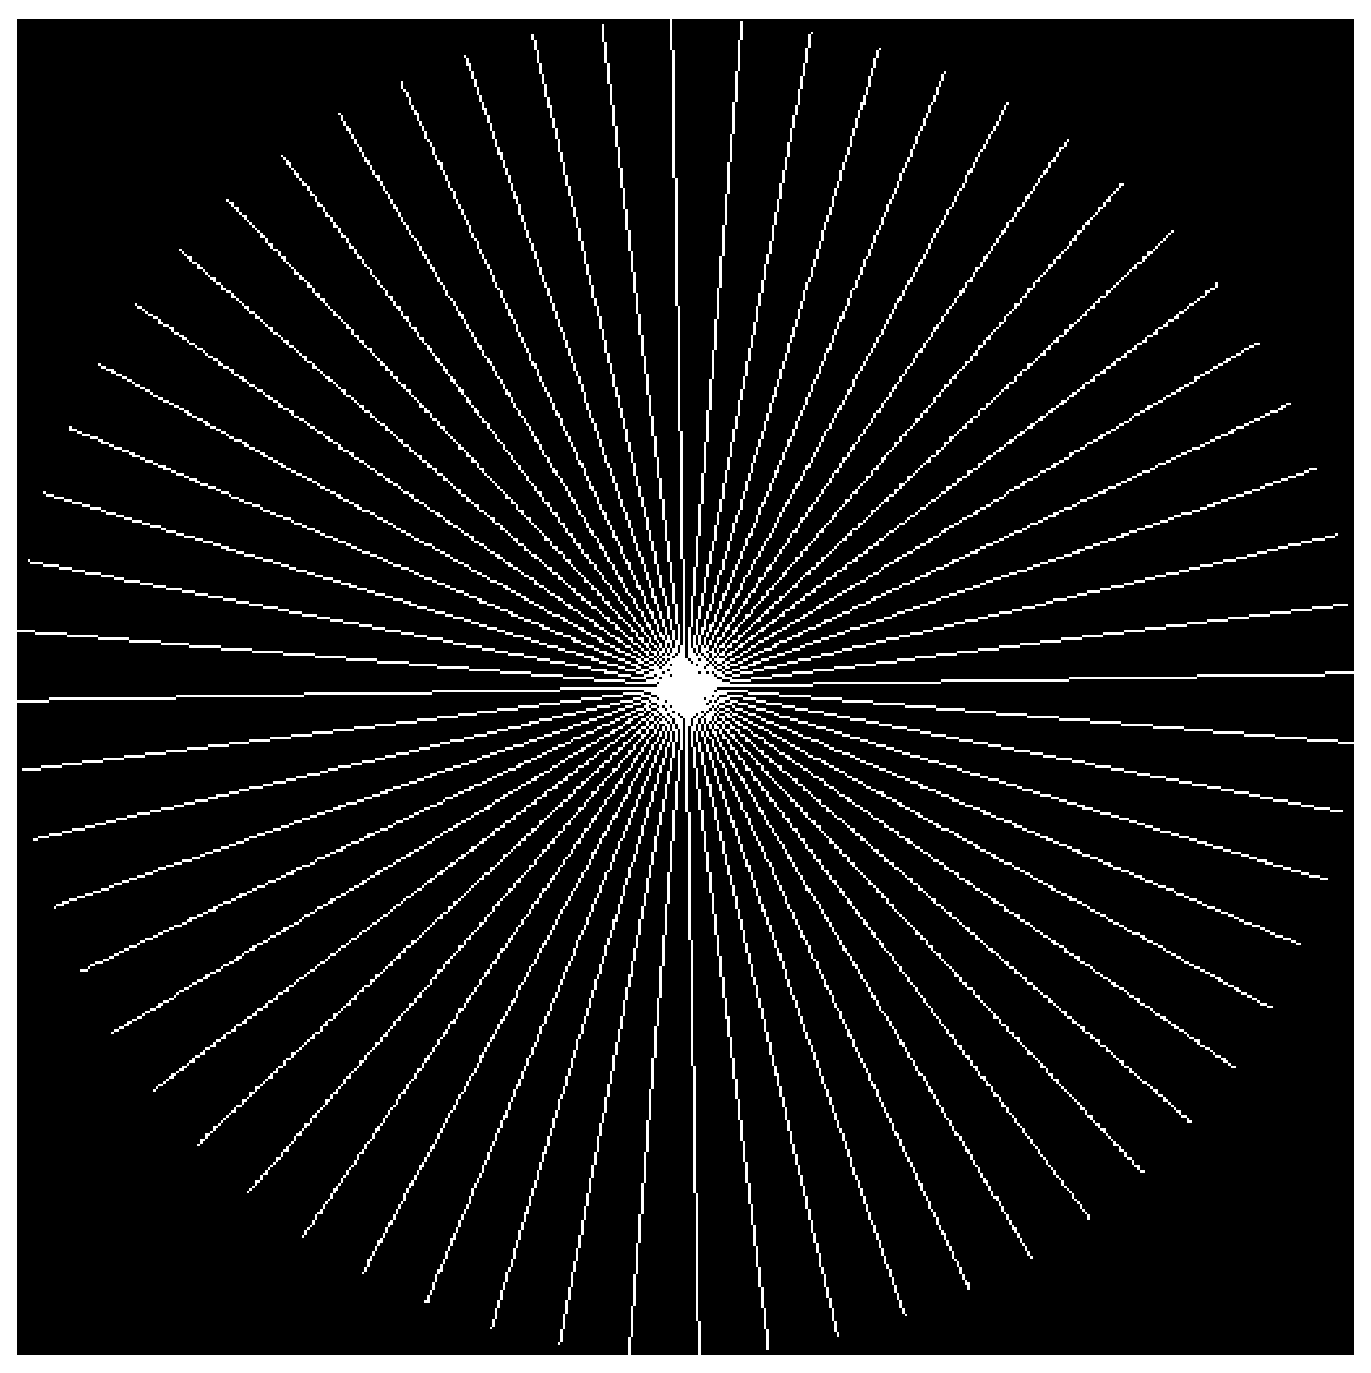
\includegraphics[width=\textwidth]{../img/intro/pradial.eps}
%\\ 动态伪随机采样(一帧)
%\end{minipage}
%\begin{minipage}[t]{0.3\textwidth}
%\centering
%\includegraphics[width=\textwidth]{../img/intro/cartesian.png}
%\\ 动态Cartesian采样(一帧)
%\end{minipage}
%\end{figure}
%		\item 评价方法为信噪比(SER)和相似性测度(SSIM)
%	\end{itemize}
%\end{frame}

\begin{frame}
	\frametitle{数值实验结果}
%	\begin{center}
	\scalebox{0.8}{
	\begin{minipage}{1\linewidth}
\begin{table}
	\centering
	\caption{各个模型在不同数据上的重建结果(伪随机采样)}
	\begin{tabular}{|c|c|c|c|c|c|c|}
		\hline
		\hline
		\multicolumn{2}{|c|}{\diagbox{模型}{数据集}}& 躯干体模 & 心脏灌注 & 胸部1 & 胸部2 & 胸部3\\	
		\hline
		\multirow{2}{*}{Zerofilled}
		&SER & 20.54 & 14.80 & 11.32 & 11.57 & 14.85\\
		\cline{2-7}&SSIM & 0.8321 & 0.8855 & 0.4820 & 0.5897 & 0.7086\\
		\hline
		\multirow{2}{*}{kt-SLR}
		&SER & \textbf{33.35} & 17.58 & 17.42 & 13.61 & 18.38\\
		\cline{2-7}&SSIM & 0.9880 & 0.9412 & 0.7712 & 0.6956 & 0.8461\\
		\hline
		\multirow{2}{*}{kt-RPCA}
		&SER & 29.27 & 18.33 & 19.31 & 14.82 & 19.81\\
		\cline{2-7}&SSIM & 0.9700 & 0.9447 & 0.8857 & 0.7920 & 0.9068\\
		\hline
		\multirow{2}{*}{L+S}
		&SER & 27.99 & 19.12 & 17.60 & 14.74 & 19.91\\
		\cline{2-7}&SSIM & 0.9514 & 0.9490 & 0.7675 & 0.7319 & 0.8791\\
		\hline
		\multirow{2}{*}{ICTGV}
		&SER & 26.88 & 17.87 & 16.31 & 12.18 & 16.84\\
		\cline{2-7}&SSIM & 0.9435 & 0.9405 & 0.6735 & 0.6080 & 0.7693\\
		\hline
		\multirow{2}{*}{Proposed}
		&SER & 32.74 & \textbf{19.57} & \textbf{20.56} & \textbf{16.24} & \textbf{21.08}\\
		\cline{2-7}&SSIM & \textbf{0.9917} & \textbf{0.9514} & \textbf{0.9402} & \textbf{0.9091} & \textbf{0.9356}\\
		\hline
	\end{tabular}
	\label{tab:result3}
\end{table}
\end{minipage}
\hspace{1.35cm}
\begin{minipage}{0.2\linewidth}
	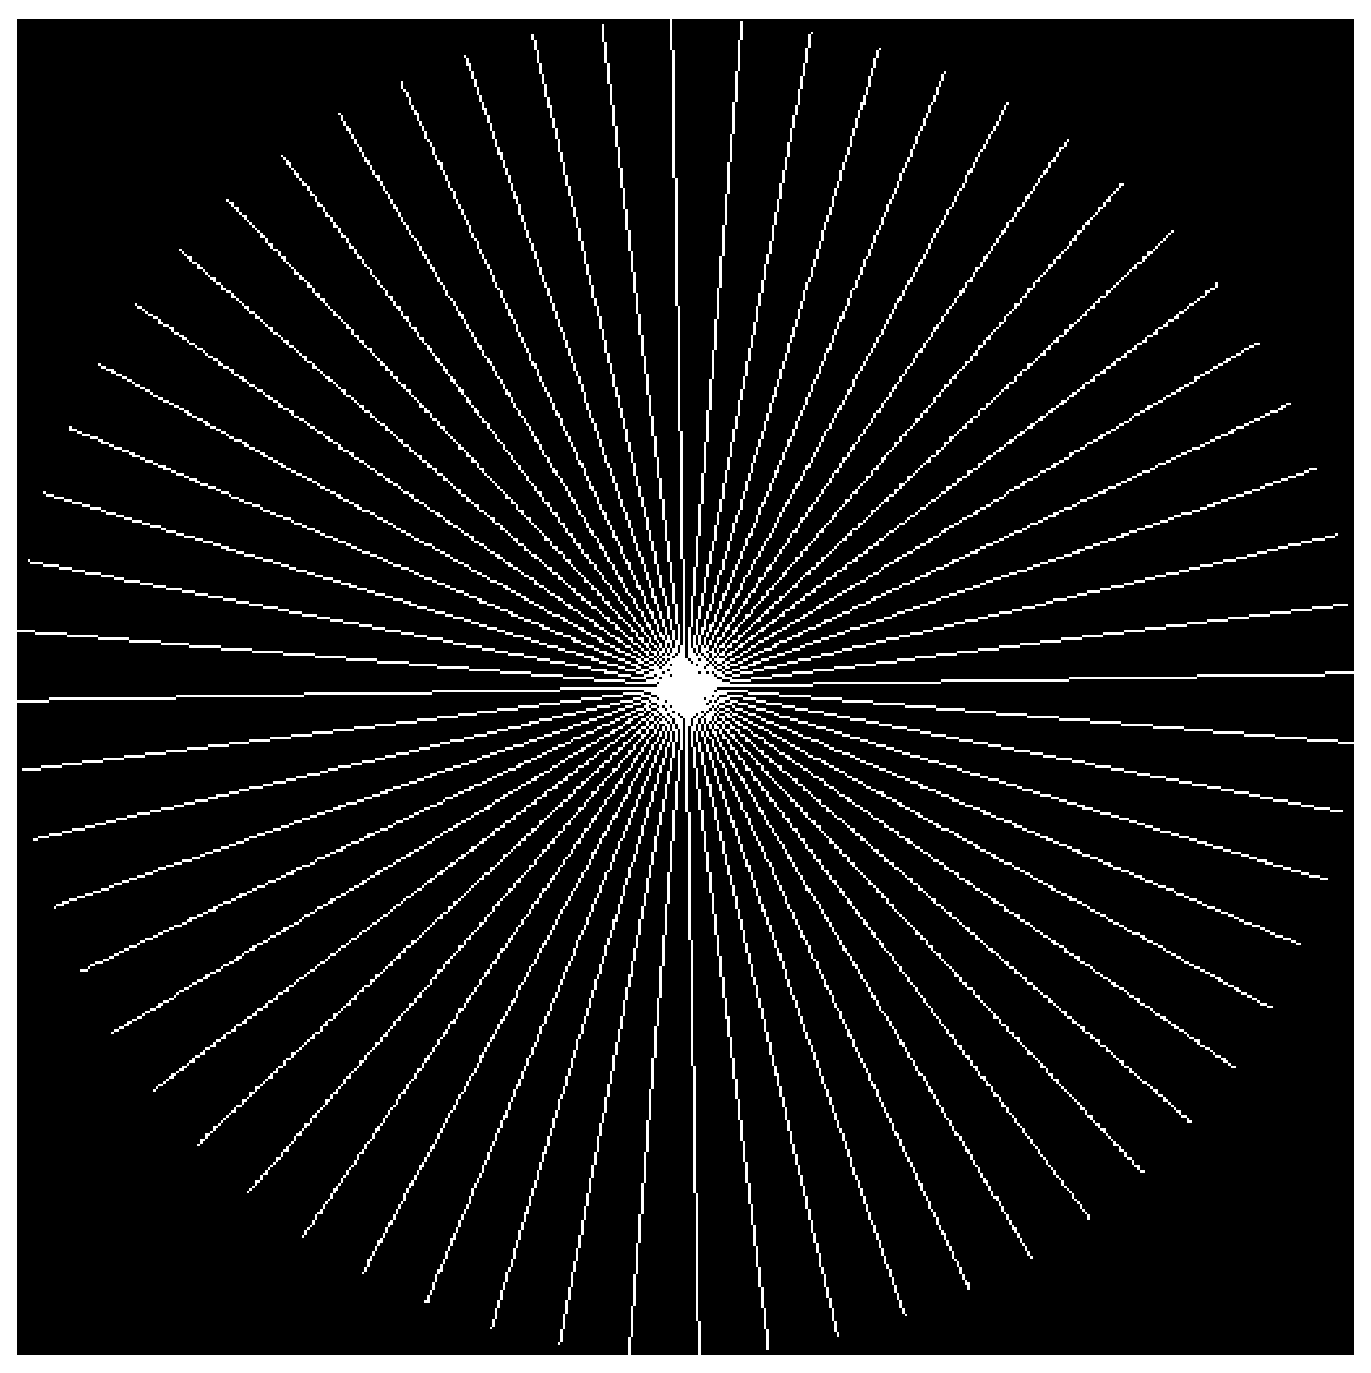
\includegraphics[width=\textwidth]{../img/intro/pradial.eps}
\end{minipage}}
%\end{center}
\end{frame}

\begin{frame}
\hspace{-0.7cm}
\begin{minipage}{1\textwidth}
%	\begin{figure}[htbp]
	\centering
		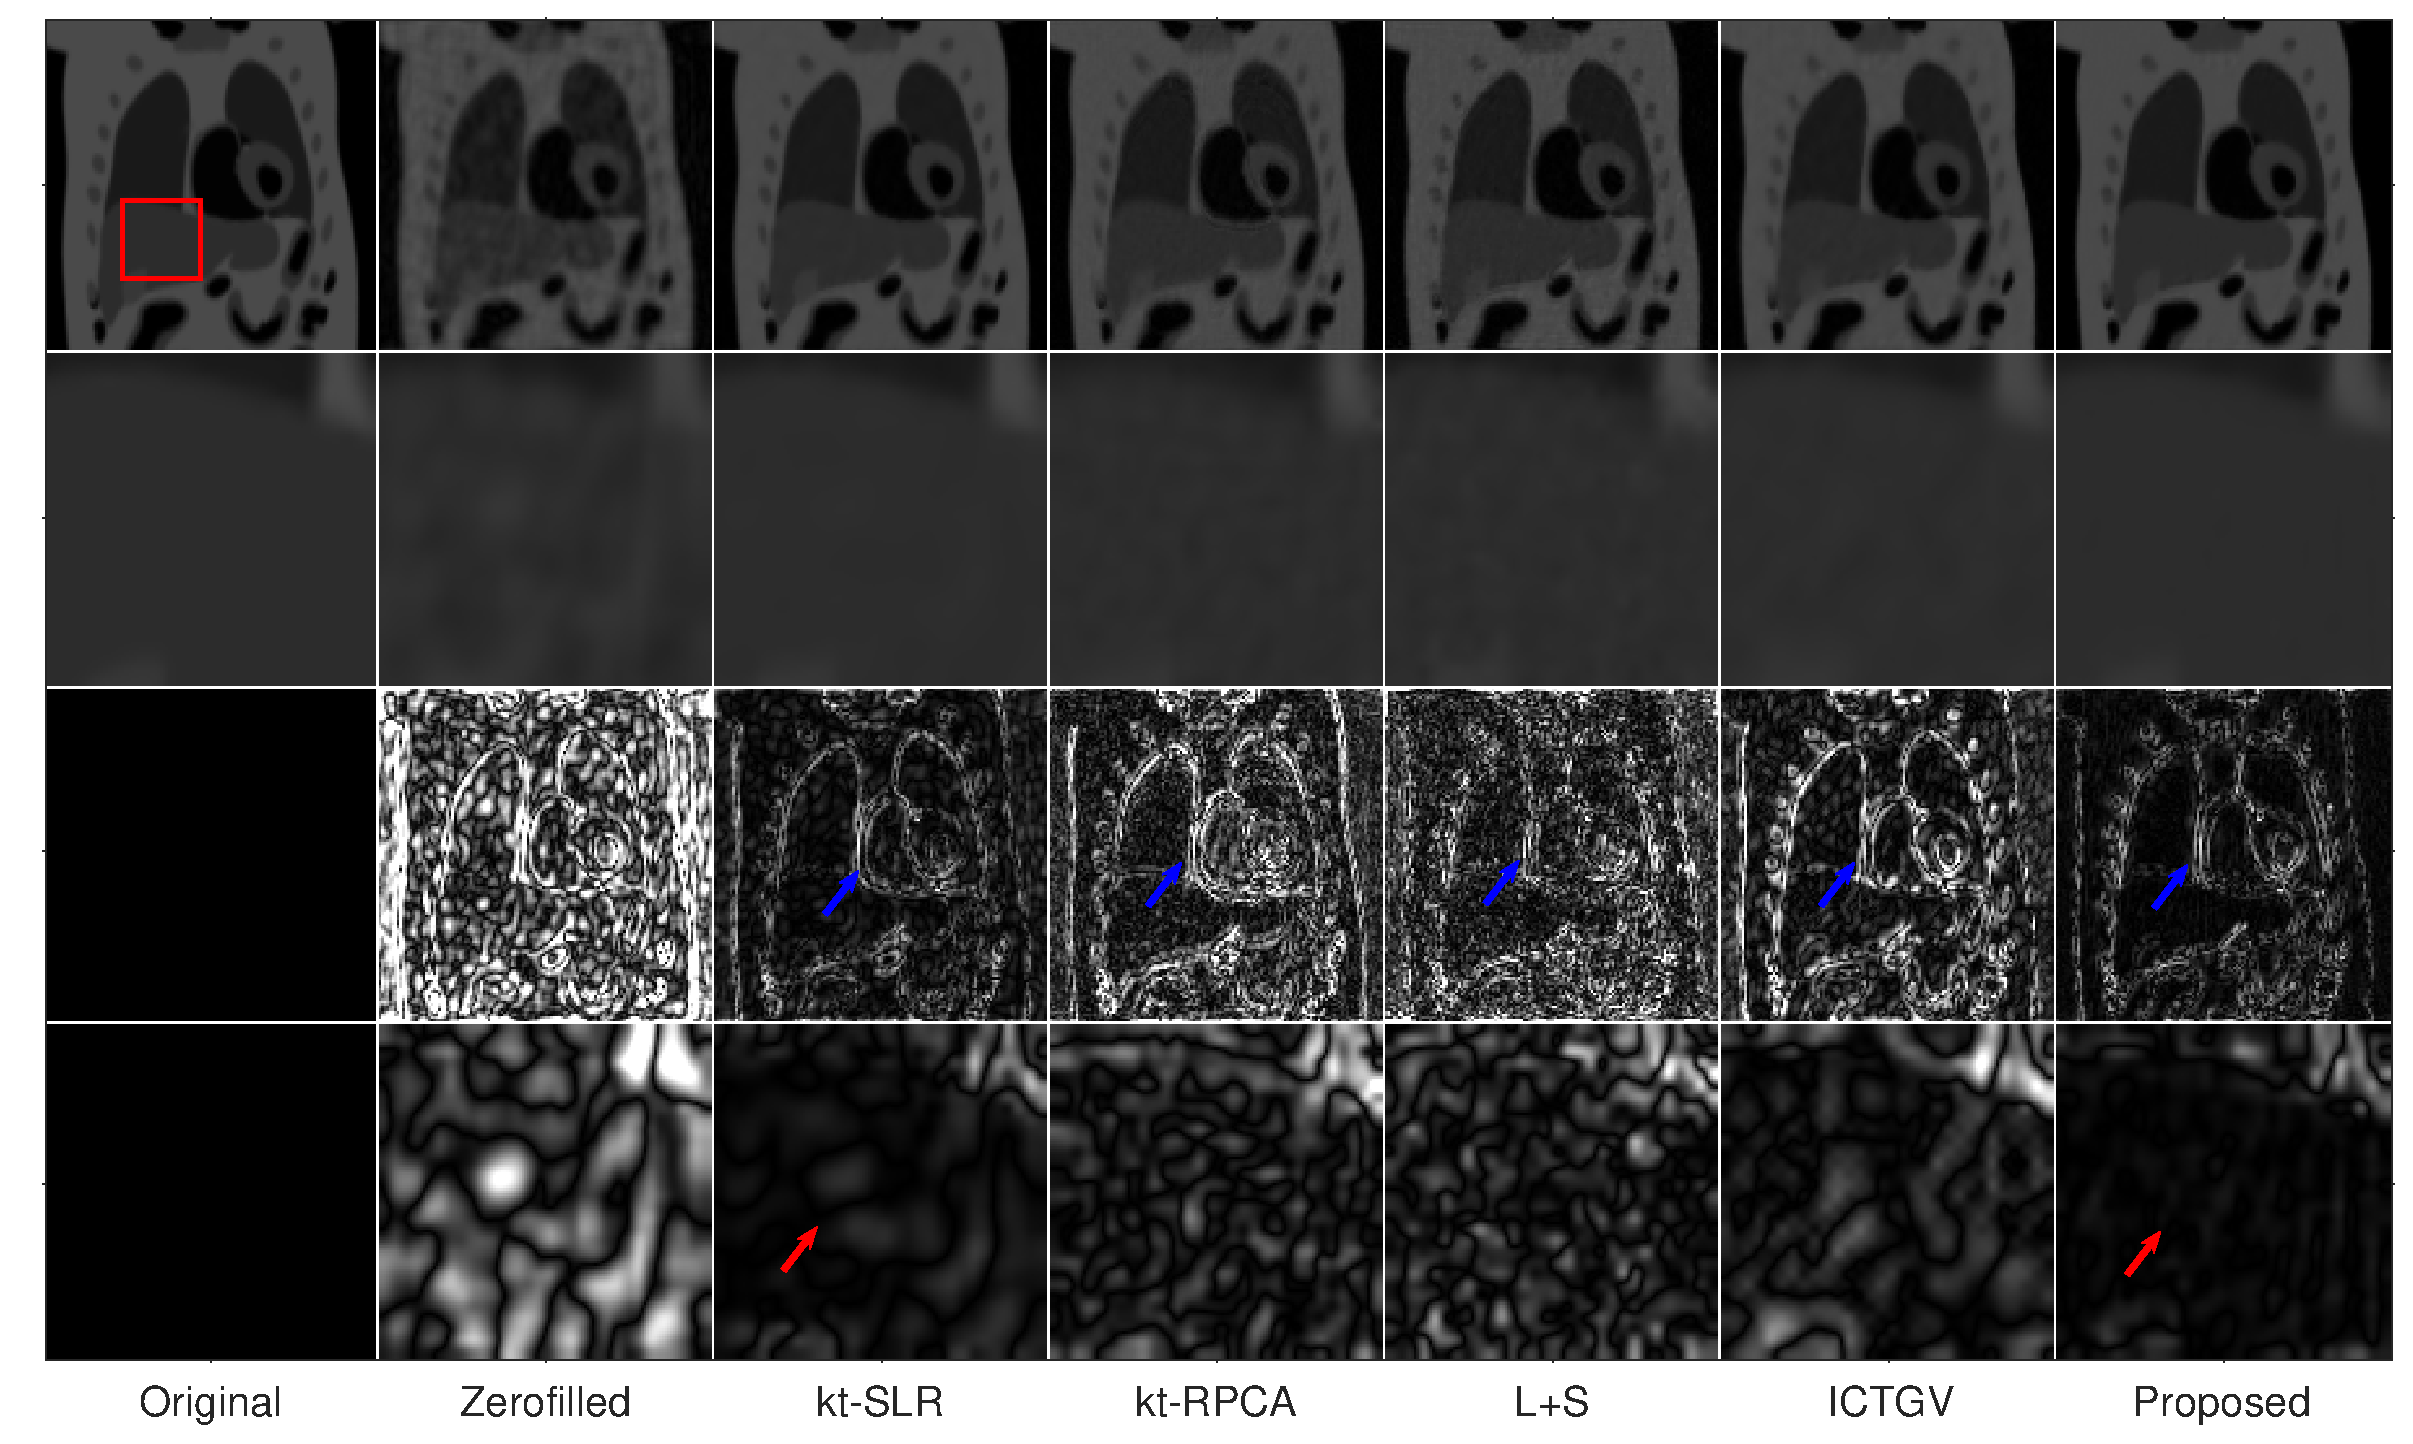
\includegraphics[width=1.1\textwidth]{../img/tgvnn/figure2_pincat.eps}
%	\caption{各个模型在躯干体模数据上的重建结果(第1帧)}
%\end{figure}
\end{minipage}
\end{frame}

%\begin{frame}
%%	\frametitle{数值实验结果}
%\hspace{-0.6cm}
%	\begin{minipage}{1\textwidth}
%	\centering
%		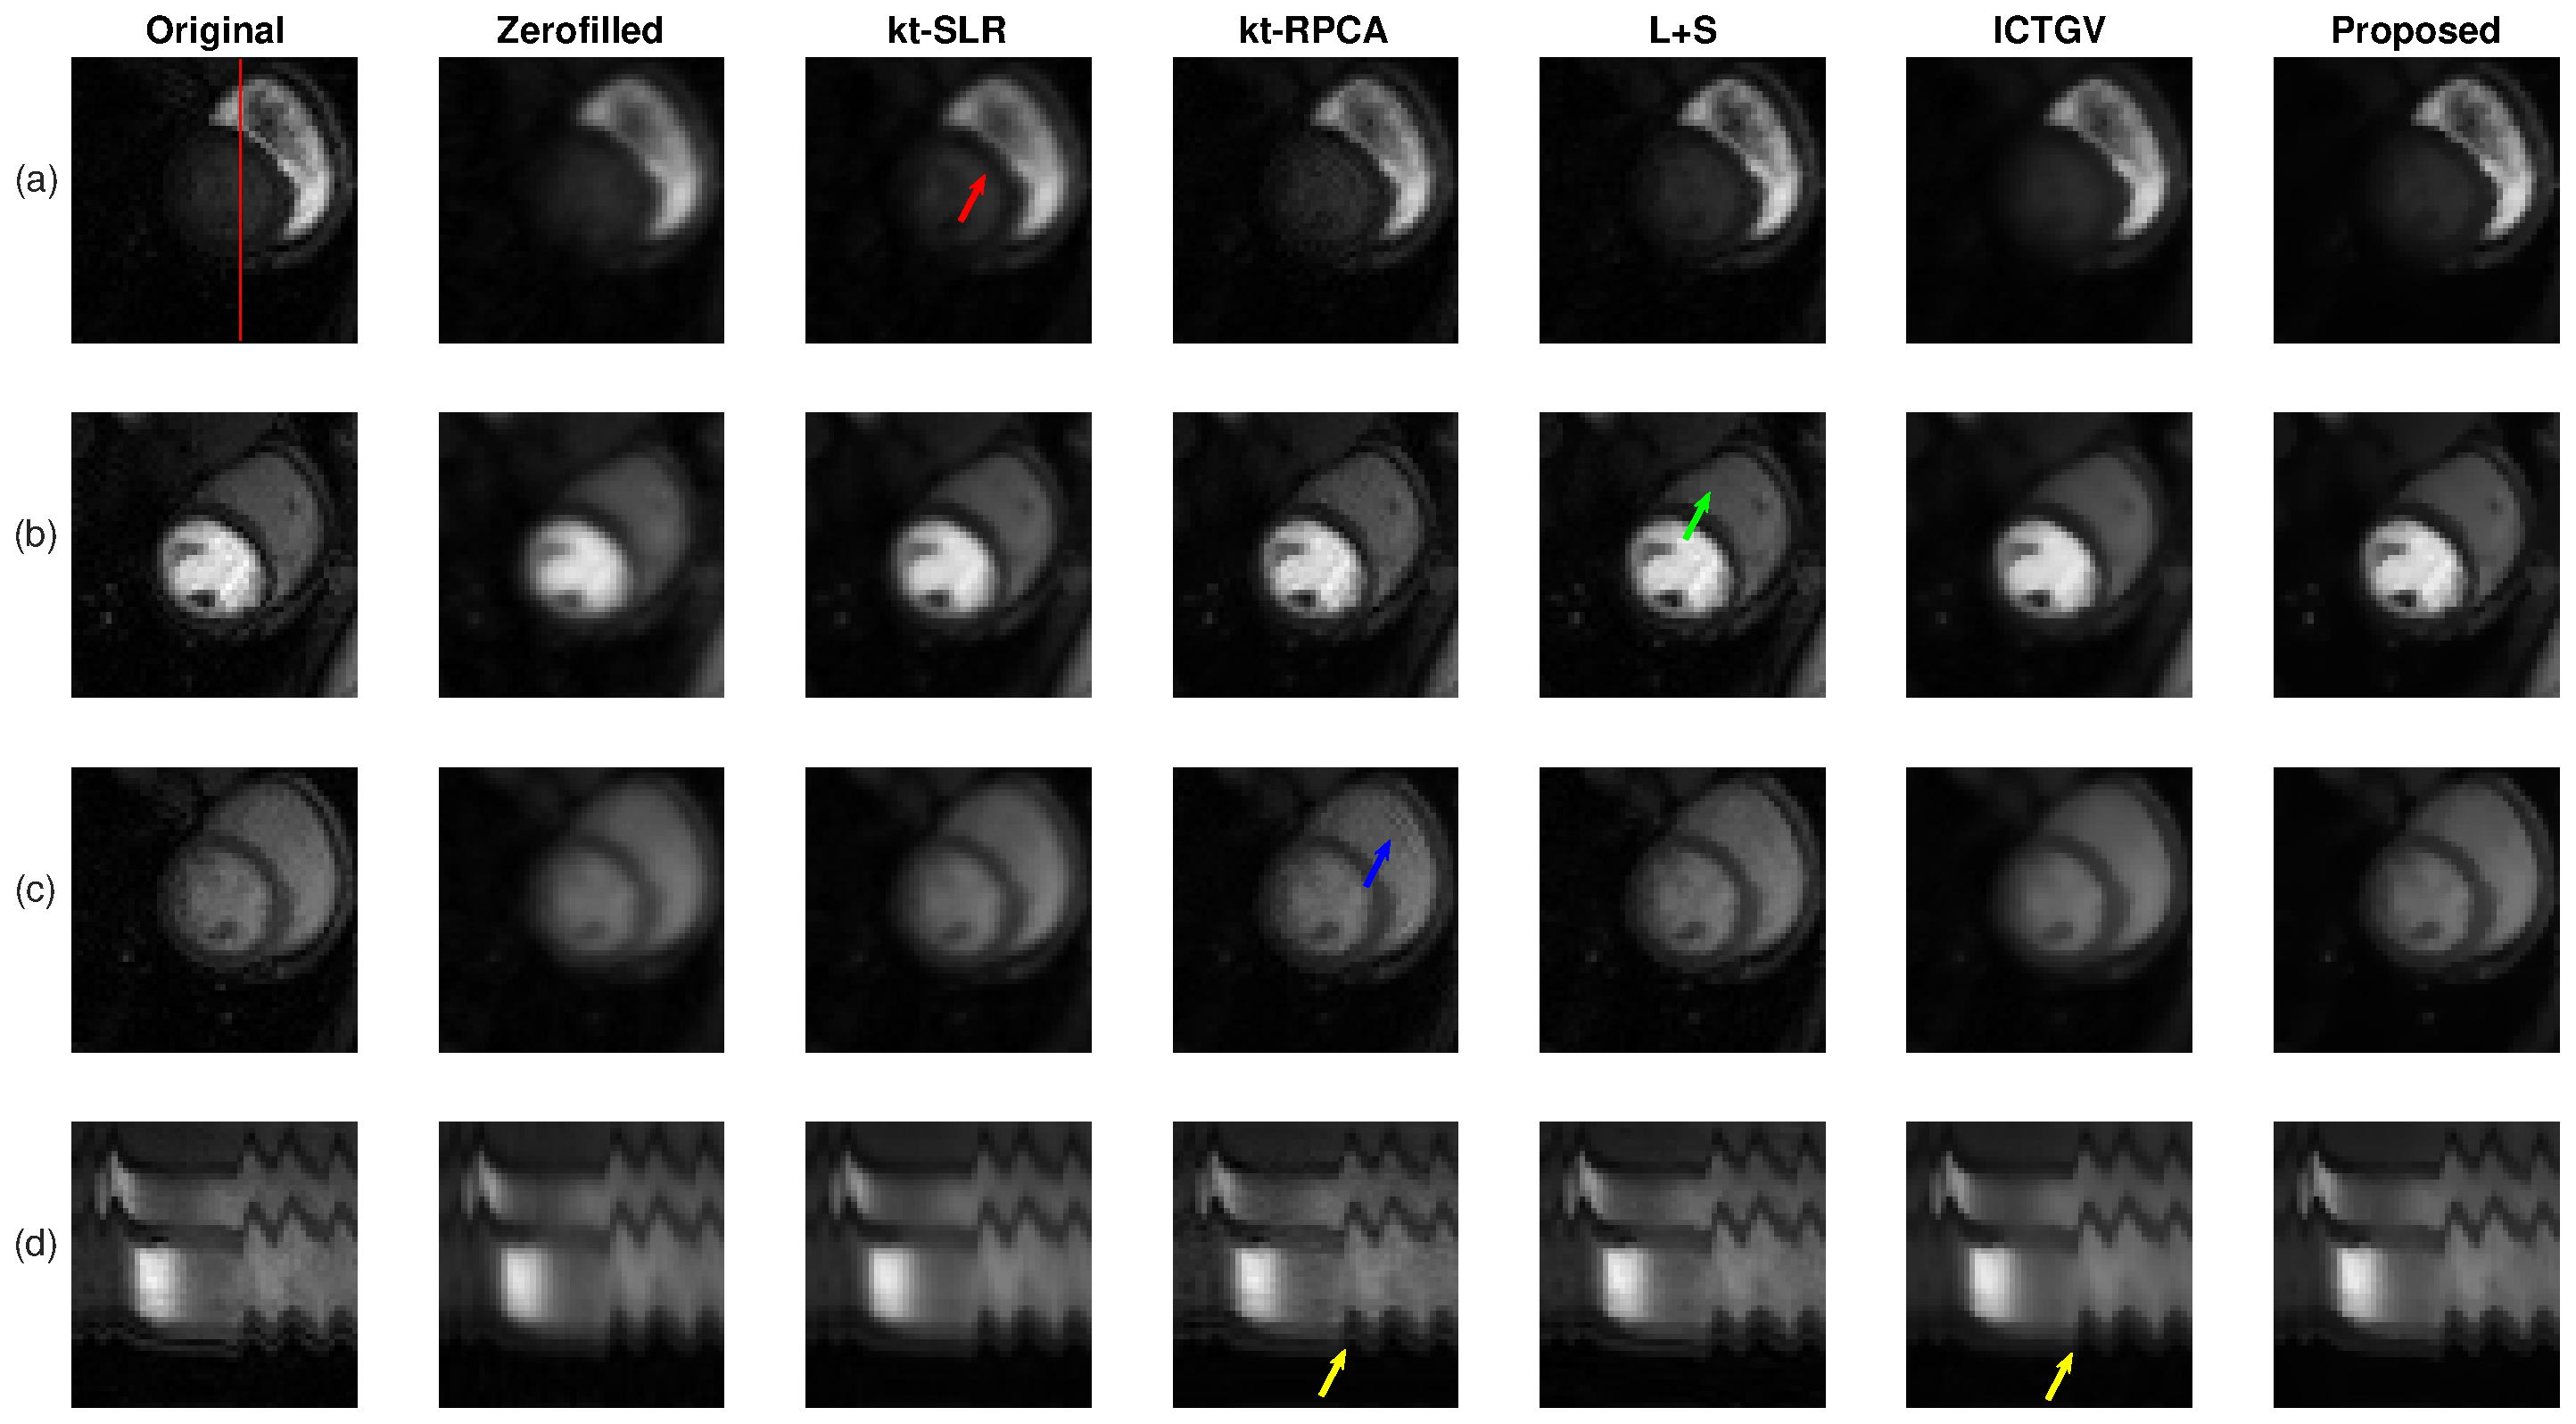
\includegraphics[width=1.1\textwidth]{../img/tgvnn/figure4_perfusion_frames.eps}
%%	\caption{各个模型在心脏灌注数据上的重建结果(时间方向)}
%\end{minipage}
%\end{frame}

\begin{frame}
%	\frametitle{数值实验结果}
\begin{minipage}{1\textwidth}
\centering
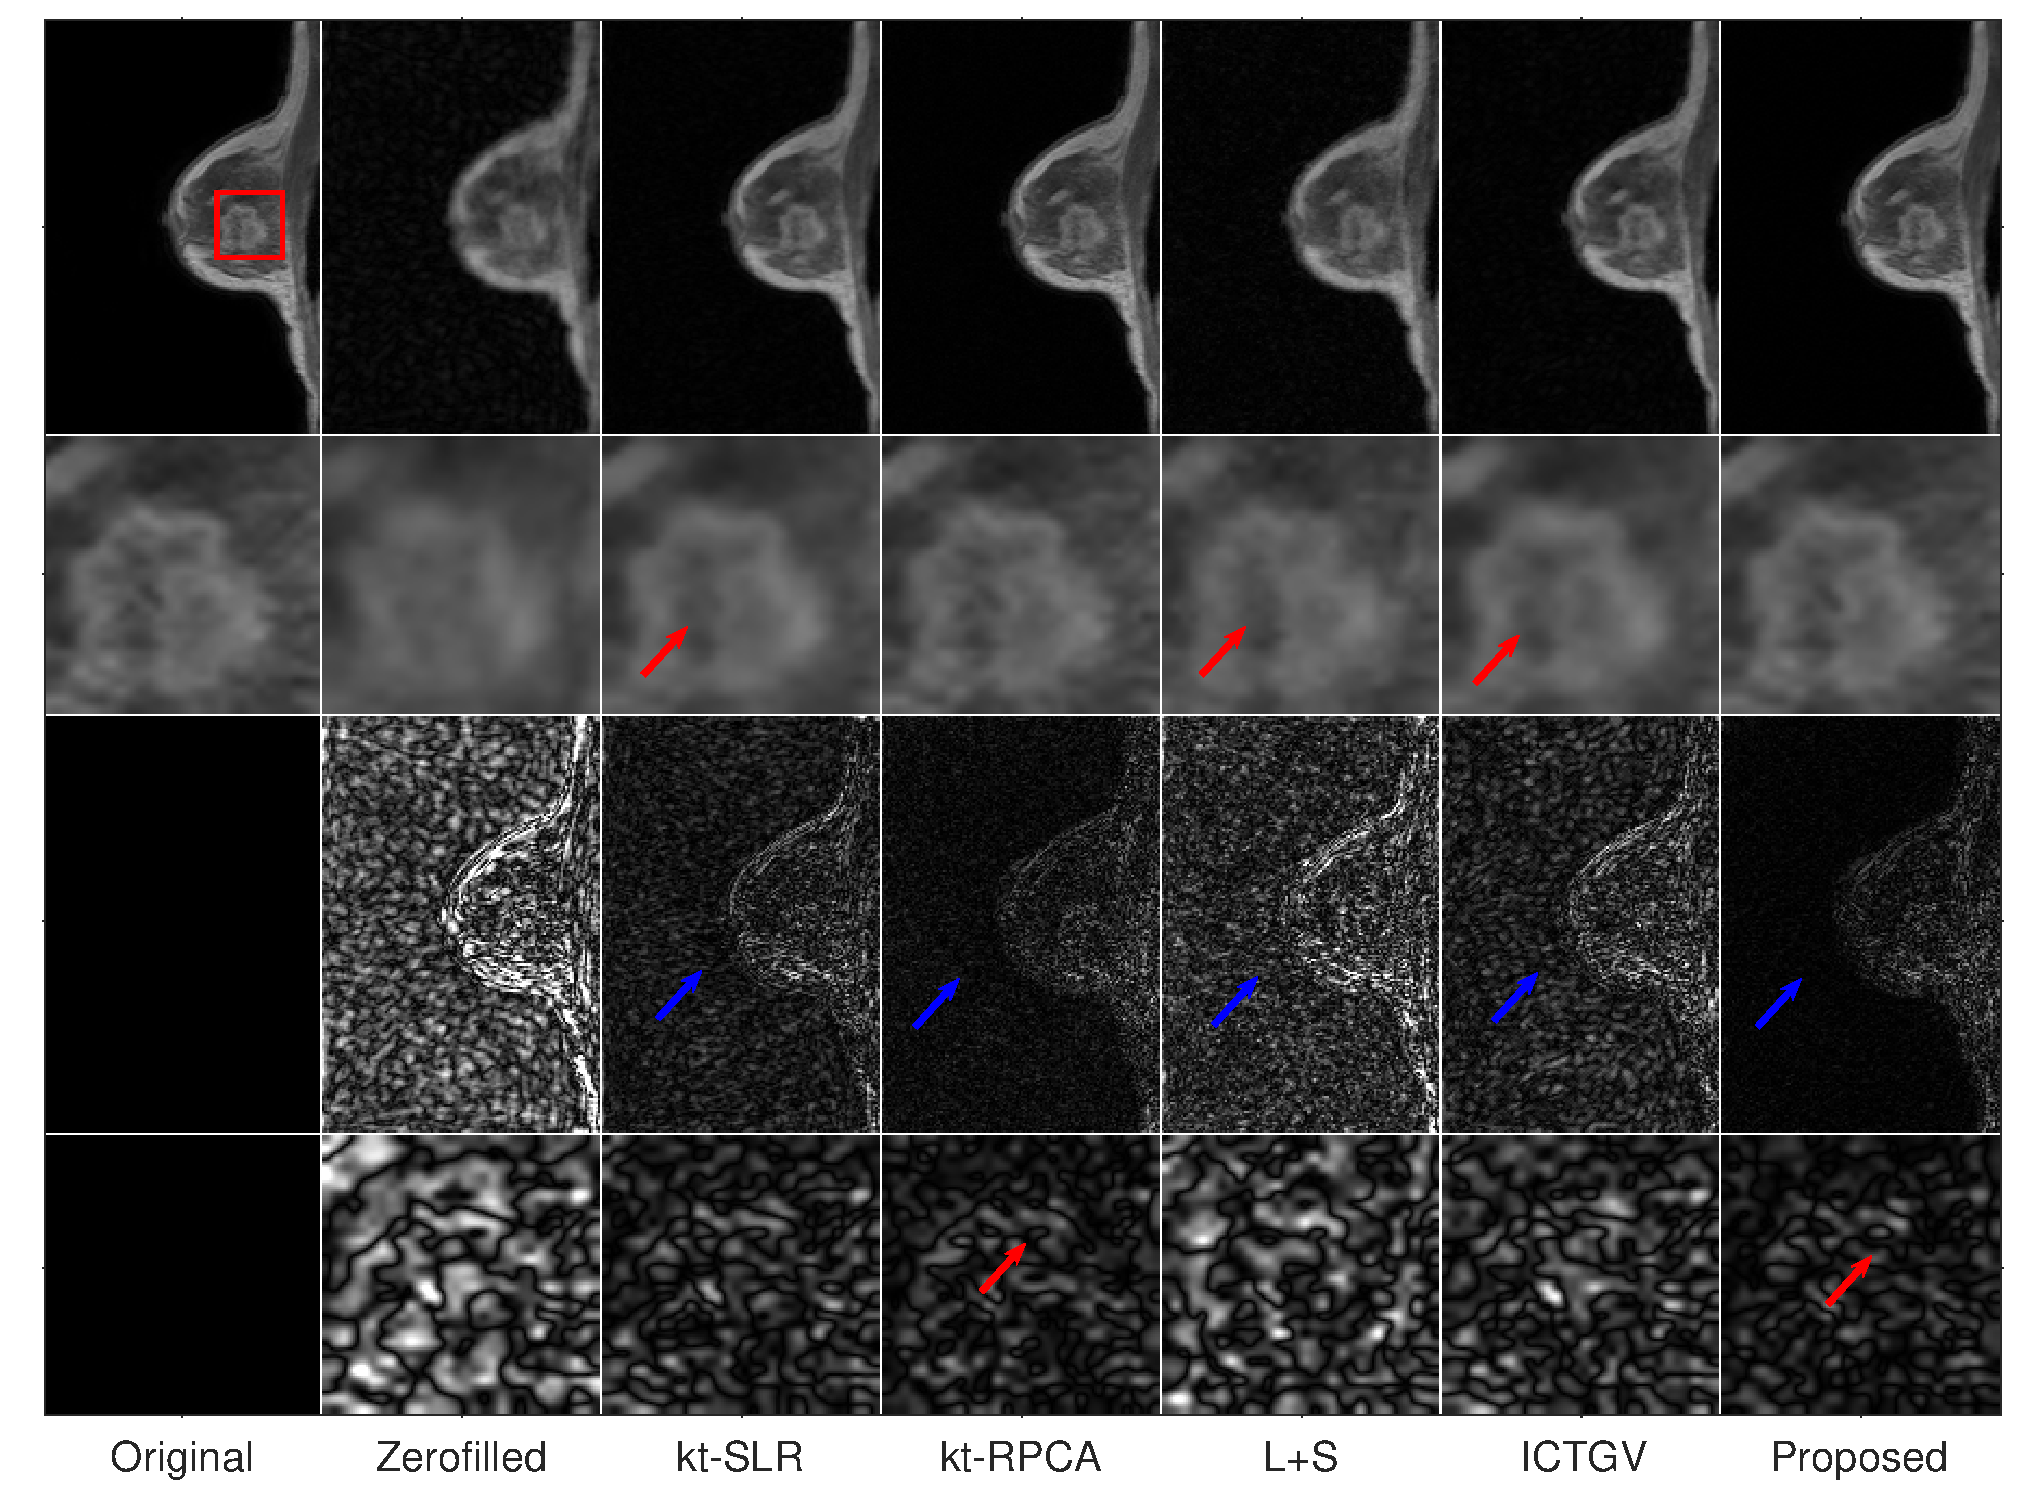
\includegraphics[width=0.9\textwidth]{../img/tgvnn/figure5_breast1.eps}
%\caption{各个模型在Breast1上的重建结果(第105帧)}
\label{fig:breast1}
\end{minipage} 
\end{frame}

\begin{frame}
\hspace{-0.9cm}
	\begin{minipage}{1\textwidth}
\centering
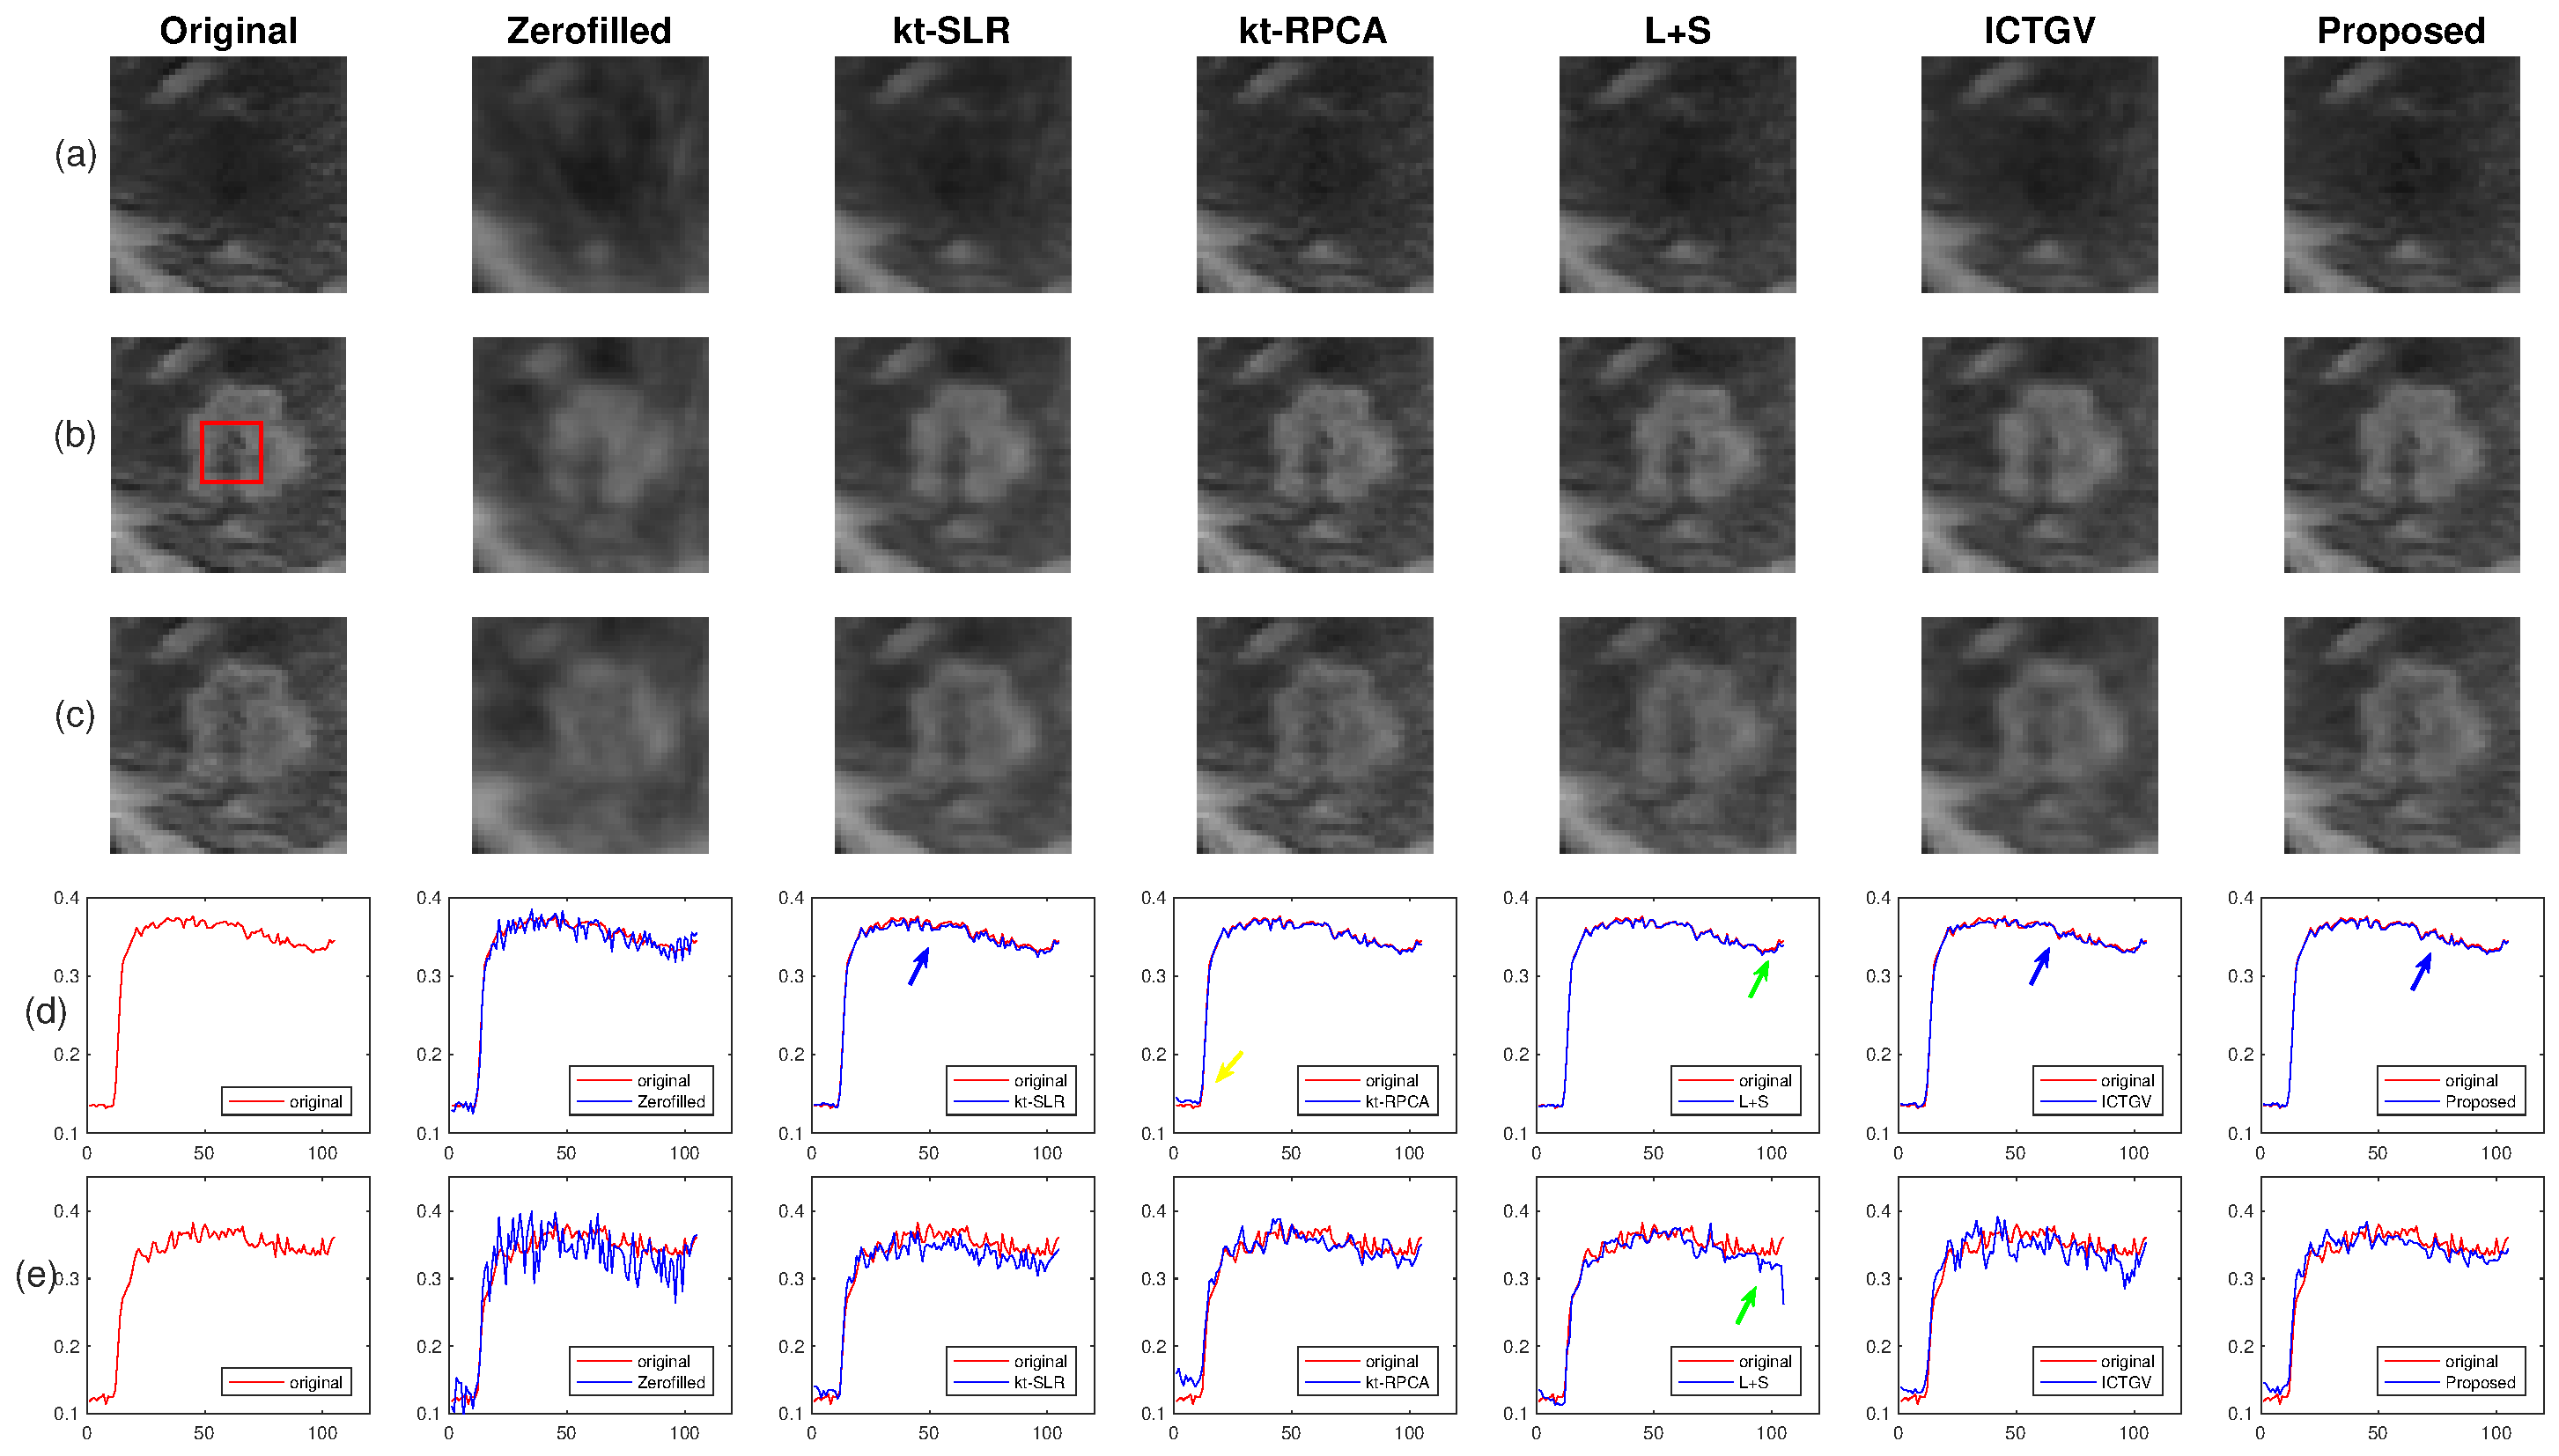
\includegraphics[width=1.15\textwidth]{../img/tgvnn/figure6_breast1_frames.eps}
%\caption{各个模型在Breast1上的重建结果(时间方向)}
\label{fig:breast1_time}
\end{minipage}
\end{frame}

\begin{frame}
%	\frametitle{数值实验结果}
%	\begin{center}
	\scalebox{0.85}{
	\begin{minipage}{1\linewidth}
\begin{table}
	\centering
	\caption{各个模型在不同加速因子下在胸部1数据上的重建结果}
	\begin{tabular}{|c|c|c|c|c|c|c|}
		\hline
		\hline
		\multicolumn{2}{|c|}{\diagbox{模型}{采样线}} & 12 & 22 & 32 & 42 & 52\\	
		\hline
		\multirow{2}{*}{Zerofilled}
		&SER & 5.98 & 9.06 & 11.32 & 12.93 & 14.33 \\
		\cline{2-7}&SSIM & 0.3218 & 0.4108 & 0.4820 & 0.5350 & 0.5818 \\
		\hline
		\multirow{2}{*}{kt-SLR}
		&SER & 15.16 & 16.10 & 17.42 & 19.07 & 19.11 \\
		\cline{2-7}&SSIM & 0.7323 & 0.7312 & 0.7712 & 0.8087 & 0.7989 \\
		\hline
		\multirow{2}{*}{kt-RPCA}
		&SER & 13.10 & 17.74 & 19.31 & 20.26 & 21.13 \\
		\cline{2-7}&SSIM & 0.6241 & 0.8356 & 0.8857 & 0.9061 & 0.9245 \\
		\hline
		\multirow{2}{*}{L+S}
		&SER & 12.75 & 16.00 & 17.60 & 18.73 & 19.64 \\
		\cline{2-7}&SSIM & 0.5885 & 0.7119 & 0.7675 & 0.8018 & 0.8275 \\
		\hline
		\multirow{2}{*}{ICTGV}
		&SER & 13.56 & 15.30 & 16.31 & 17.03 & 17.56 \\
		\cline{2-7}&SSIM & 0.6001 & 0.6485 & 0.6735 & 0.6895 & 0.7007\\
		\hline
		\multirow{2}{*}{Proposed}
		&SER & \textbf{16.49} & \textbf{19.06} & \textbf{20.56} & \textbf{21.82} & \textbf{22.96}\\
		\cline{2-7}&SSIM & \textbf{0.8620} & \textbf{0.9119} & \textbf{0.9402} & \textbf{0.9535} & \textbf{0.9632}\\
		\hline
	\end{tabular}
	\label{tab:sampling}
\end{table}
\end{minipage}
\hspace{0.4cm}
\begin{minipage}{0.2\linewidth}
	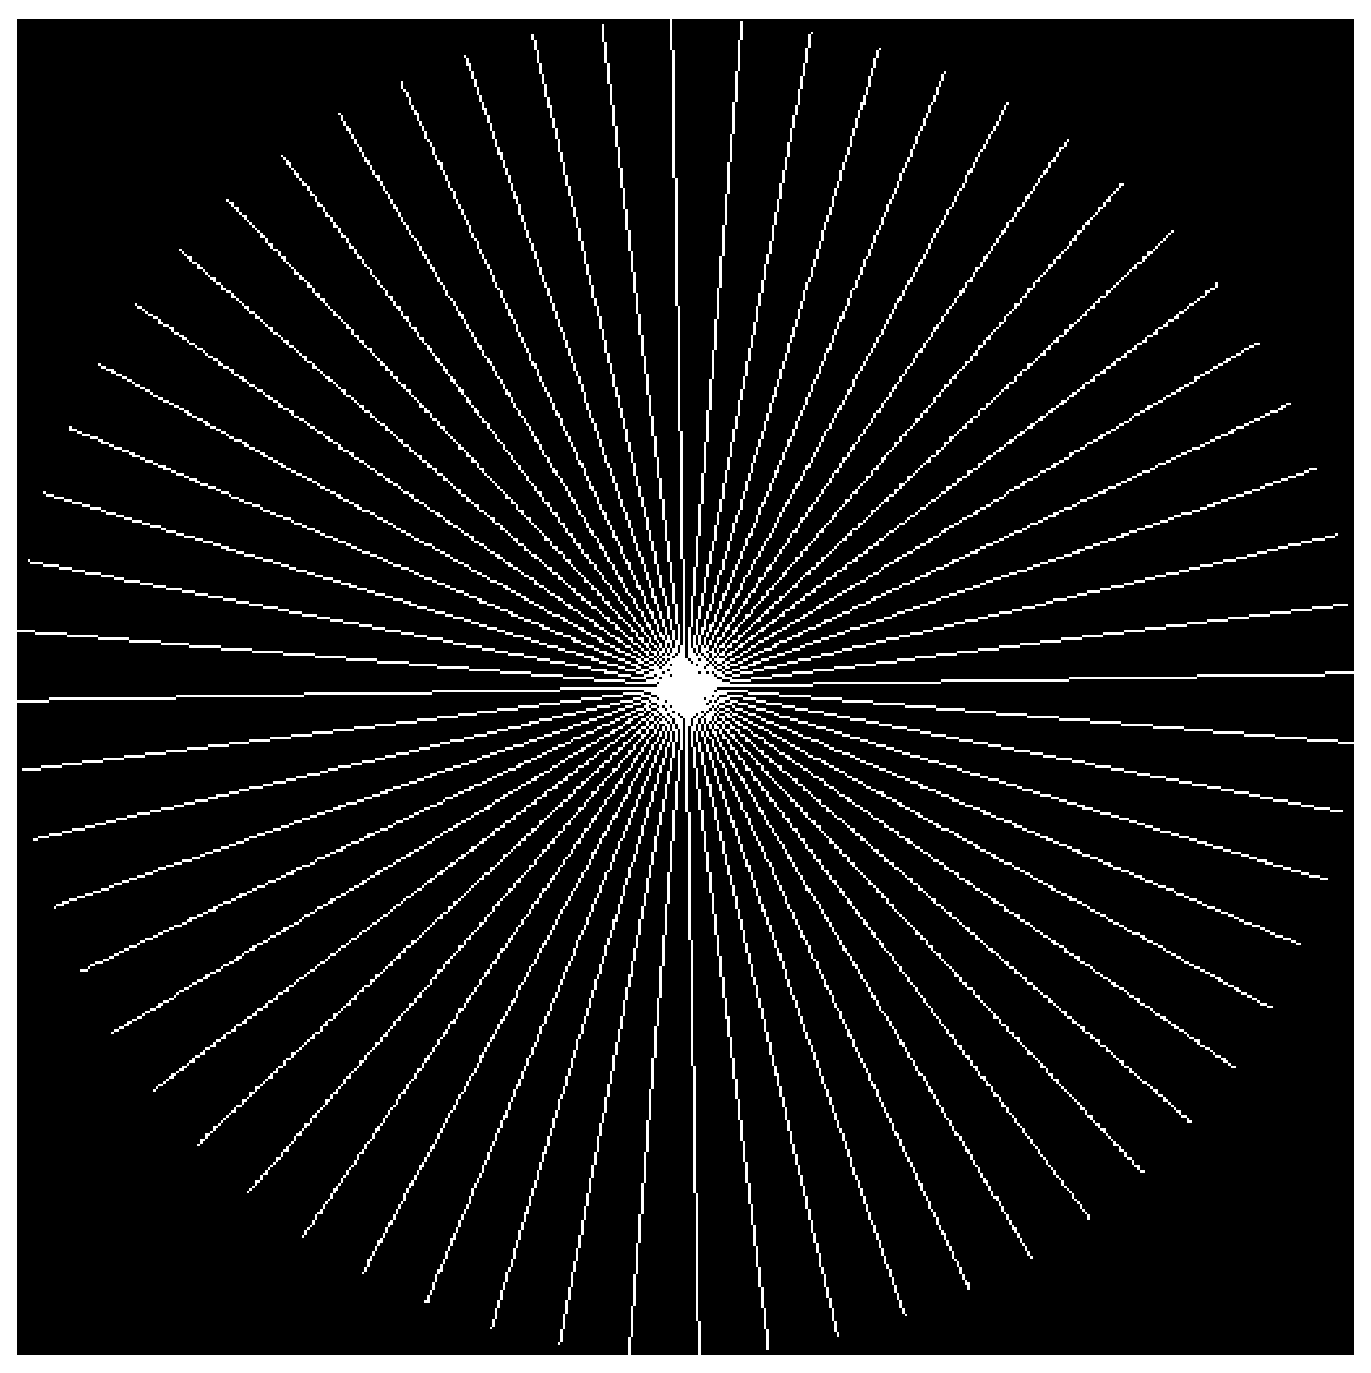
\includegraphics[width=\textwidth]{../img/intro/pradial.eps}
\end{minipage}}
%\end{center}
\end{frame}


\begin{frame}
%	\frametitle{数值实验结果}
%	\begin{center}
	\scalebox{0.8}{
	\begin{minipage}{1\linewidth}
	\centering
\begin{table}
\centering
\caption{各个模型在胸部1数据上的重建结果(Cartesian采样)}
\begin{center}
\begin{tabular}{|l|l|l|l|l|l|l|}
\hline
\hline
模型 & Zerofilled & kt-SLR & kt-RPCA & L+S & ICTGV & Proposed \\
\hline
SER & 11.29 & 16.60 & 16.86 & 14.55 & 14.33 & \textbf{17.79} \\
\hline
SSIM & 0.7370 & 0.8942 & 0.9126 & 0.8379 & 0.7681 & \textbf{0.9169}\\
\hline
\end{tabular}
\end{center}
\label{tab:cartesian}
\end{table}
\end{minipage}
\hspace{0.8cm}
\begin{minipage}{0.23\linewidth}
	\includegraphics[width=\textwidth]{../img/intro/cartesian.png}
\end{minipage}}

\scalebox{0.8}{
	\begin{minipage}{1\linewidth}
	\centering
\begin{table}
\centering
\caption{各个模型在胸部1数据上运行时间比较}
\begin{center}
\begin{tabular}{|l|l|l|l|l|l|l|}
\hline
\hline
\multirow{2}{*}{模型} & kt-SLR & kt-RPCA & L+S & ICTGV & Proposed & Proposed \\
& (CPU) & (CPU) & (CPU) & (CPU) & (CPU) & (GPU) \\
\hline
时间 (s) & 5794.88 & 641.71 & 493.80 & 2572.04 & 2812.90 & \textbf{28.35} \\
\hline
\end{tabular}
\end{center}
\label{tab:time3}
\end{table}
\end{minipage}}
%\end{center}
\end{frame}

%------------------------------------------------
\section{胸部DCE-MRI压缩感知重建模型中时间稀疏正则项的量化评估}
%------------------------------------------------
%\AtBeginSection[]
%{
    \begin{frame}
        \tableofcontents[currentsection,hideallsubsections]
    \end{frame}
%}

\subsection{胸部DCE-MRI的定量参数}
\begin{frame}
%	\frametitle{时间稀疏项}
	\begin{itemize}
		\item DCE-MRI通过测量注入造影剂期间和之后的信号,使得图像的每个体素产生一个时间强度曲线,用于定量地估计生理参数,例如体积转移常数($K^{trans}$) 和血管外细胞体积分数 ($v_e$) 等。
		\begin{figure}[htbp]
\begin{minipage}[t]{0.3\textwidth}
\centering
\includegraphics[width=\textwidth]{ktrans.png}
\\ $K^{trans}$
\end{minipage}
\hspace{1cm}
\begin{minipage}[t]{0.3\textwidth}
\centering
\includegraphics[width=\textwidth]{ve.png}
\\ $v_e$
\end{minipage}
\end{figure}
		\item 定量的参数有助于给医生提供客观的标准,从而减少了主观性,起到了帮助癌症诊断、评估和治疗的作用。
%		\item 因此,对于DCE-MRI,体素的时间强度曲线决定了参数估计的准确性,即高时间分辨率有利于提精确地定量分析。
	\end{itemize}
\end{frame}

%\begin{frame}
%%	\frametitle{时间稀疏项}
%	\begin{itemize}
%		\item 虽然压缩感知已经应用于胸部DCE-MRI中,但目前还没有研究通过量化分析的方式来比较时间方向的稀疏项在DCE-MRI中的表现
%		\item 因此对于定量胸部DCE-MRI,不同时间方向的稀疏项对重建误差的影响是未知的
%	\end{itemize}
%\end{frame}

\subsection{时间方向稀疏正则项的量化评估}
\begin{frame}
%	\frametitle{时间方向稀疏正则项的量化评估}
	\begin{itemize}
		\item 在将压缩感知理论应用于临床肿瘤成像之前,其可靠性和准确性的研究是必要的。
		\item \textbf{首次}通过量化分析的方式比较和评估五种不同的时间方向的稀疏变换$\Phi$在压缩感知模型中的表现,分别为:
		\begin{equation}
		\begin{aligned}
	 \mathrm{FT}:\quad &\min_X\frac{1}{2}||AX-B||_{\mathrm{F}}^2 + \alpha||\mathcal{F}_tX||_1 \\
%	\vspace{0.1cm}
	 \mathrm{WT}:\quad &\min_X\frac{1}{2}||AX-B||_{\mathrm{F}}^2 + \alpha||\mathcal{W}_tX||_1 \\
%	\vspace{0.1cm}
	 \mathrm{TV}:\quad &\min_X\frac{1}{2}||AX-B||_{\mathrm{F}}^2 + \alpha||\nabla_t X||_1 \\
%	\vspace{0.1cm}
	 \mathrm{TGV}:\quad &\min_X\frac{1}{2}||AX-B||_{\mathrm{F}}^2 + \alpha||\mathrm{TGV}(X)||_1 \\
%	\vspace{0.1cm}
	 \mathrm{NN}:\quad &\min_X\frac{1}{2}||AX-B||_{\mathrm{F}}^2 + \alpha||X||_*
\end{aligned}
\end{equation}
	\end{itemize}
\end{frame}

%\begin{frame}
%	\frametitle{时间稀疏项}
%	\begin{itemize}
%		\item 图像大小$192\times 128\times 105$
%		\item 采样模式为200个不同的Cartesian采样
%		\item 使用FISTA求解
%		\item 评价标准为图像的增强信噪比(SER)和肿瘤区域参数的一致性相关系数(CCC)
%	\end{itemize}
%\end{frame}

%\begin{frame}
%在每一帧图像上,我们对低频区域进行全采样,对高频区域进行随机采样。
%\begin{figure}
%\centering
%  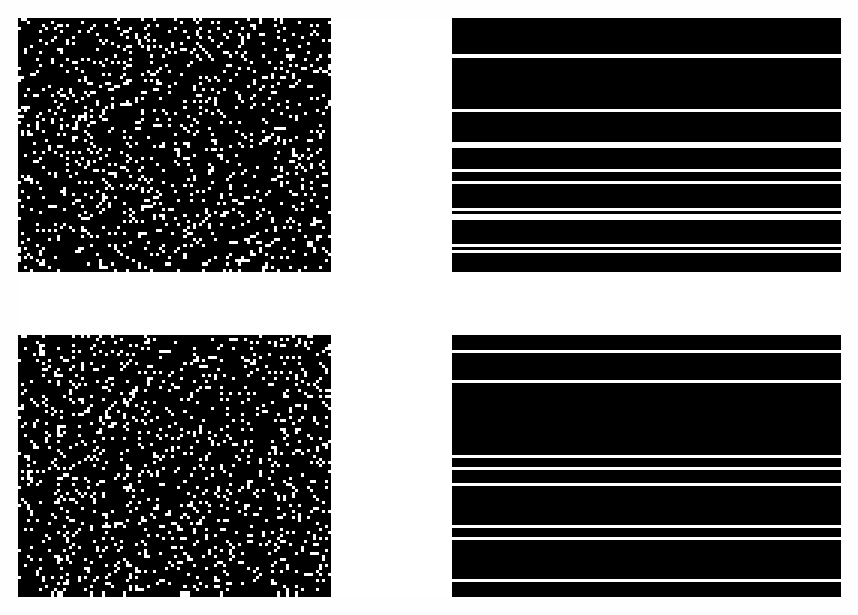
\includegraphics[width=0.6\textwidth]{../img/qetsr/figure1.eps}
%\caption{
%Cartesian采样模式的例子
%}
%\end{figure}
%\end{frame}

%------------------------------------------------
\subsection{数值实验结果与分析}
\begin{frame}
	\frametitle{数值实验设置}
	\begin{itemize}
		\item 胸部DCE-MRI图像
		\item 随机生成200个下采样率相同的Cartesian采样模式
		\item 使用FISTA算法进行图像重建
		\item 使用标准Tofts-Kely模型计算肿瘤区域$K^{trans}$与$v_e$的值
		\item 重建图像的信噪比和肿瘤区域定量参数的一致性相关系数(CCC)
	\end{itemize}
\end{frame}

\begin{frame}
\frametitle{数值实验结果}
\begin{table}
\caption{重建图像的平均SER与CCC}
\centering
\begin{tabular}{|l|l|l|l|}
\hline
\hline
\multirow{2}*{稀疏项}&\multirow{2}*{SER}&\multicolumn{2}{c|}{CCC} \\
\cline{3-4}
~ & ~ & \kt & \Ve \\
\hline
Zerofilled & 15.1 & 0.694 & 0.636\\
\hline
FT & 26.4 & 0.763 & 0.575\\
\hline
WT & 21.8 & 0.878 & 0.733\\
\hline
TV & 27.7 & \textbf{0.974} & 0.916\\
\hline
TGV$_\alpha^2$ & 27.8 & \textbf{0.974} & \textbf{0.917}\\
\hline
NN & \textbf{29.1} & 0.842 & 0.799\\

\hline
\end{tabular}
\label{tab:result}
\end{table}
\end{frame}

%\begin{frame}
%	\begin{figure}
%	\begin{minipage}[t]{0.75\linewidth}
%		\centering
%		\includegraphics[width=1\textwidth]{001.pdf}
%	\end{minipage}
%	\begin{minipage}[t]{0.75\linewidth}
%		\centering
%		\includegraphics[width=1\textwidth]{105.pdf}
%	\end{minipage}
%	\end{figure}
%\end{frame}

\begin{frame}
%	\frametitle{实验结果}
	\begin{figure}[htbp]
\centerline{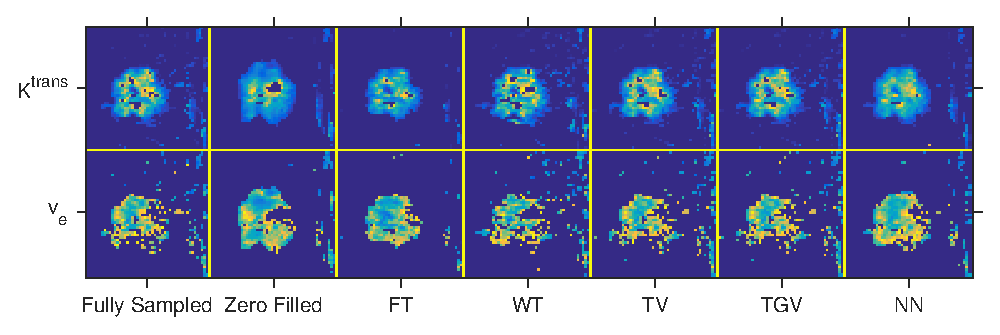
\includegraphics[width=1\textwidth]{../img/qetsr/figure4.eps}}
%\caption{肿瘤区域参数\kt 和\Ve 图像。在视觉上,TV和TGV$_{\alpha}^2$与的参数图像最接近。}
\end{figure}
\end{frame}

\begin{frame}
%	\frametitle{实验结果}
	\begin{figure}[htbp]
\centerline{\includegraphics[width=0.65\textwidth]{../img/qetsr/figure6}}
%\caption{
%全采样图像与重建图像肿瘤区域像素时间曲线的比较图。
%}
\end{figure}
\end{frame}

\begin{frame}
\begin{figure}[htbp]
\centerline{
    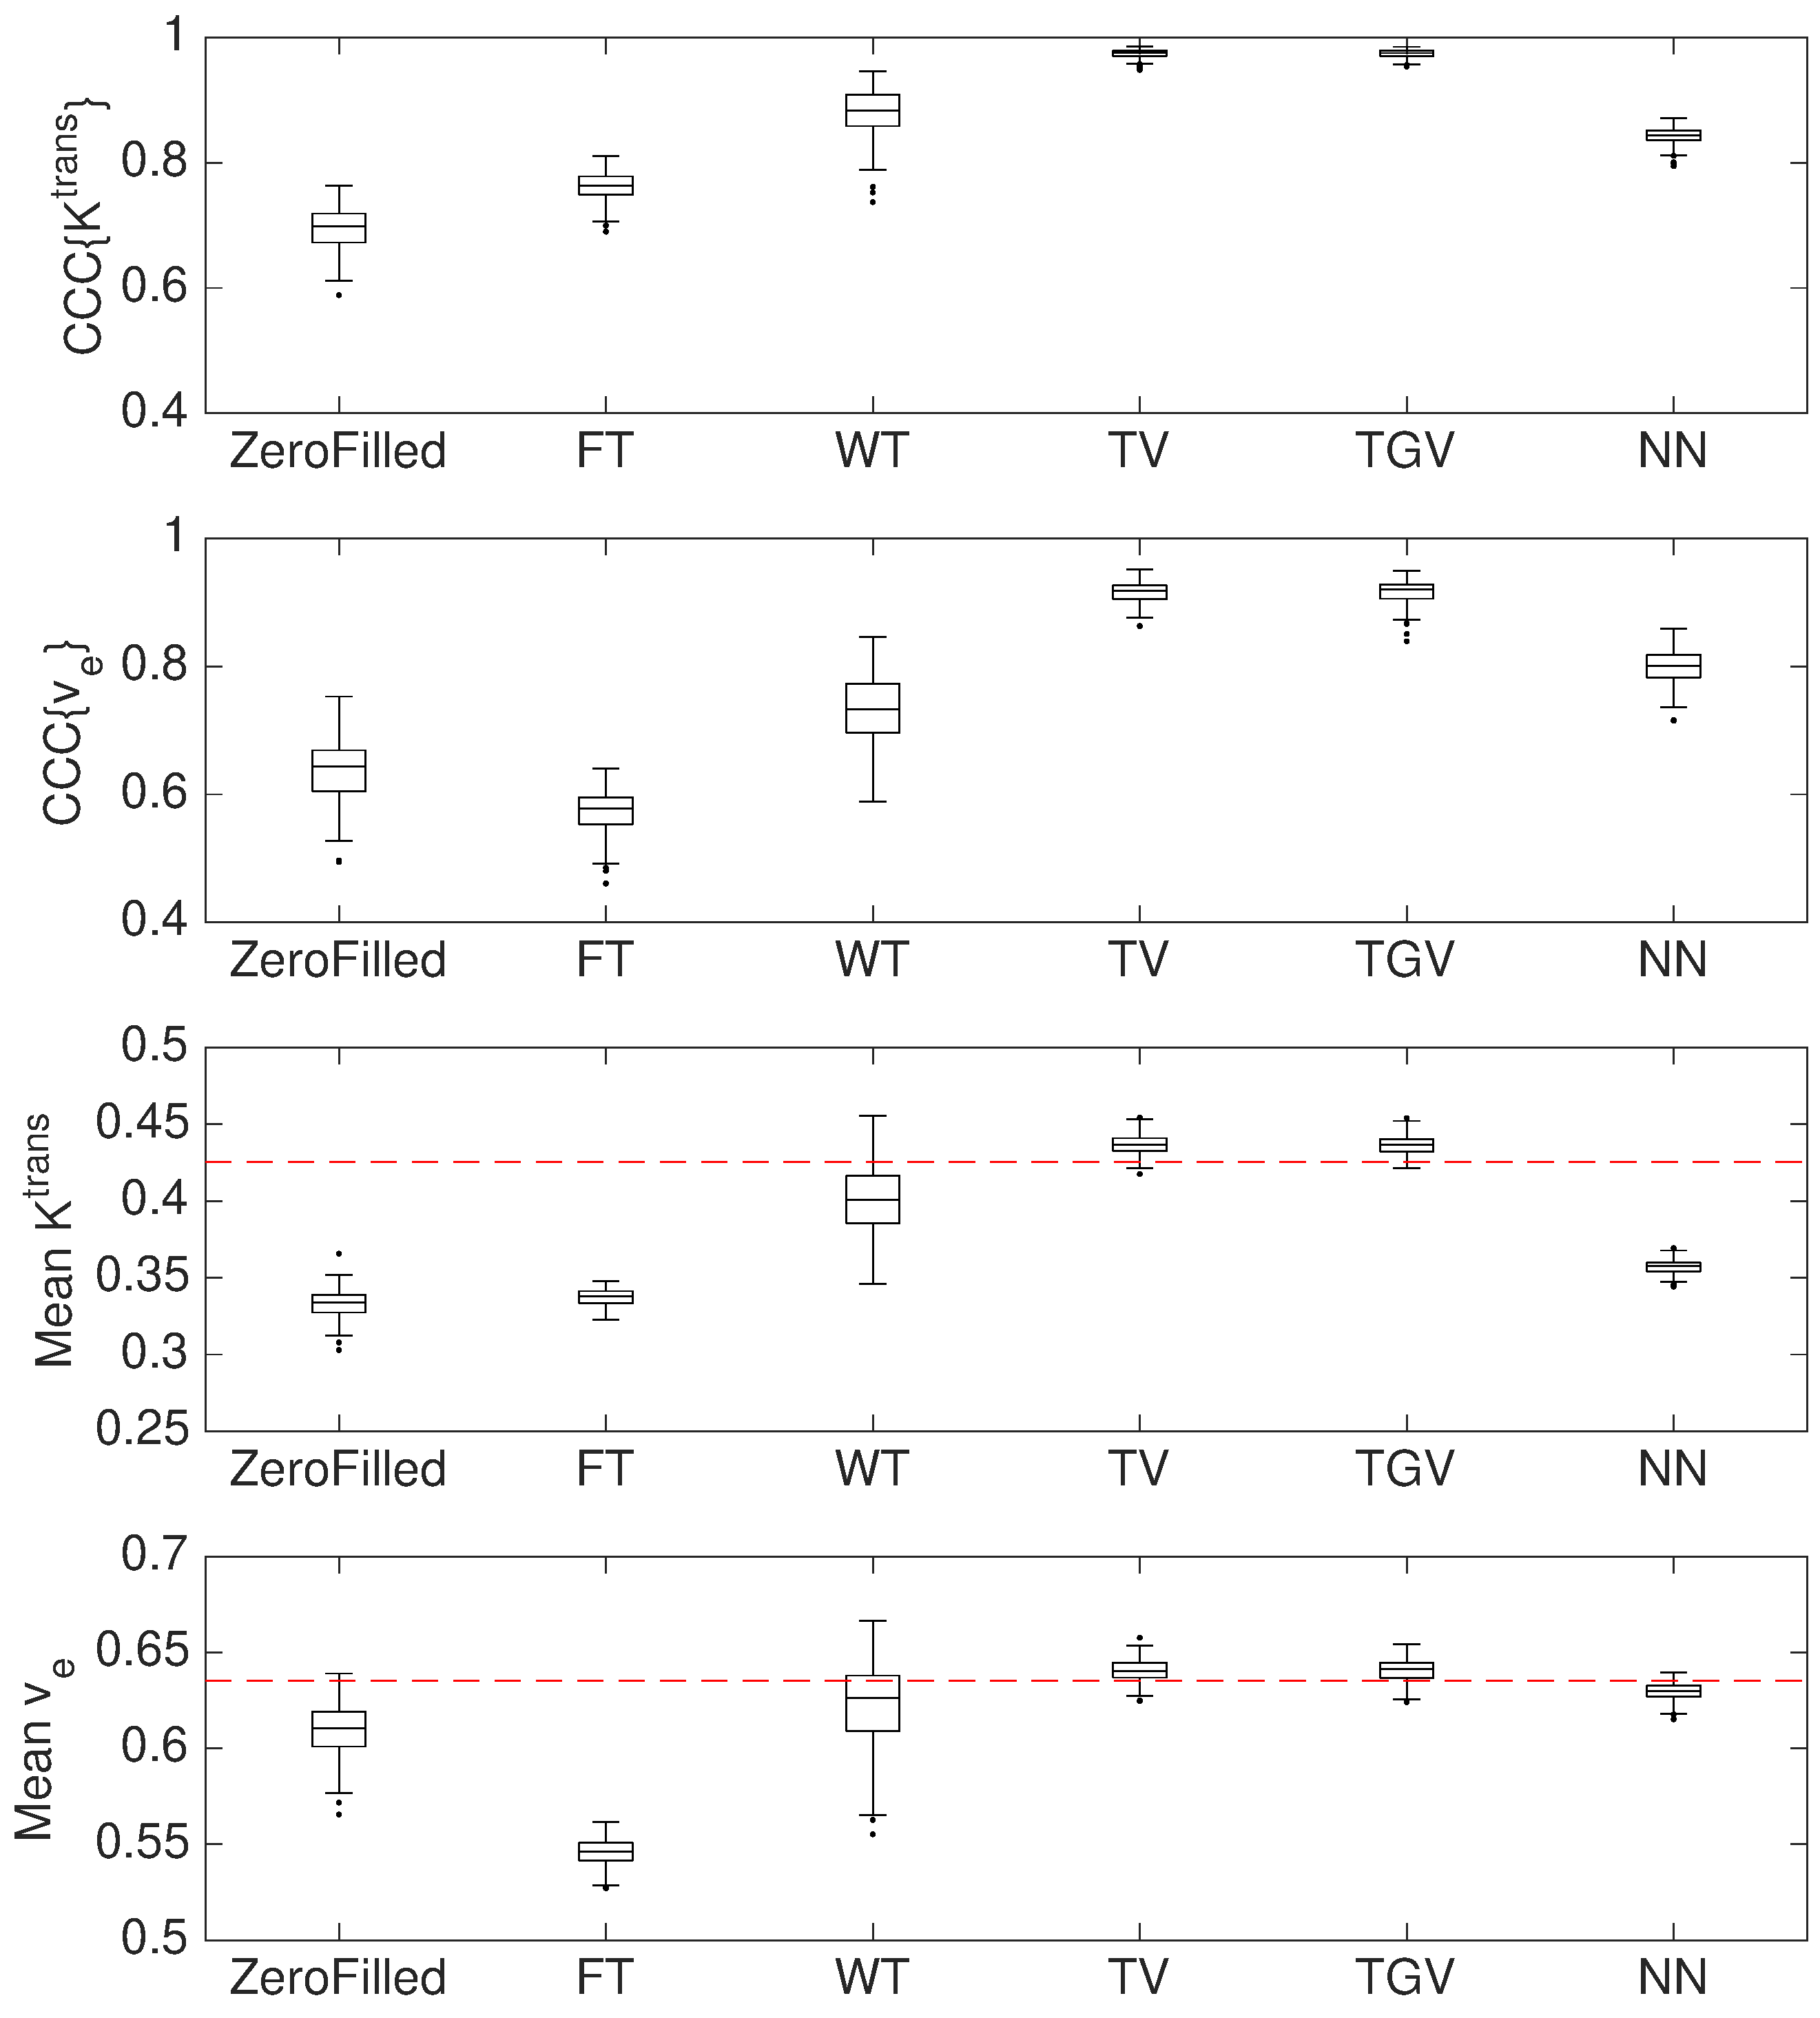
\includegraphics[width=0.6\textwidth]{../img/qetsr/figure7.eps}
}
\end{figure}
\end{frame}

\begin{frame}
	\frametitle{数值试验分析}
	对于\textbf{胸部DCE-MRI}:
	\begin{itemize}
		\item TV/TGV在统计上\textbf{没有}显著性差异
		\item TV/TGV得到了最准确的\textbf{定量分析}
		\item NN得到了最高的\textbf{信噪比}
	\end{itemize}
	\vspace{1cm}
	\textbf{结论:}对于那些需要得到更加精确整体质量的应用,最好的稀疏项选择是核范数;如果需要得到更精确的参数分析,最好的选择是TV或者TGV。
\end{frame}

%------------------------------------------------
\section{基于GPU的实时MRF字典生成与参数图重建}
%------------------------------------------------
%\AtBeginSection[]
%{
    \begin{frame}
        \tableofcontents[currentsection,hideallsubsections]
    \end{frame}
%}

\subsection{磁共振指纹成像}
\begin{frame}
%	\frametitle{磁共振指纹成像}
磁共振指纹(MRF)是一种新的定量MRI方法,可以在单次数据采集中同时获取多个组织参数,如$T_1$,$T_2$和质子密度
	\begin{minipage}{1\textwidth}
\centerline{\includegraphics[width=1.2\textwidth]{../img/intro/mrf.png}}
\end{minipage}
\end{frame}

%\begin{frame}
%\frametitle{研究背景--MRF}
%	MRF重建参数图的过程中涉及到三个步骤,分别为信号采集、预定义字典生成和模板匹配。
%	\begin{itemize}
%		\item 选取对所需参数敏感的MR序列对信号进行采样,并且序列的参数,如重复时间($T_R$)等,需要随着时间随机变动,使得不同参数的组织在MR序列中产生独特的信号演化(指纹) -- bSSFP/uSSFP ...
%		\item 字典中包含着不同参数的组织在该MR序列中的模拟演化 -- EPG/Bloch ...
%		\item 模式识别算法用来比较每个体素指纹和字典中元素的匹配度,重建参数图 -- 模板匹配、降维(SVD/grouping)、深度神经网络 ...
%	\end{itemize}
%\end{frame}

\begin{frame}
%\frametitle{研究背景--MRF}
\hspace{-1.5cm}
	\begin{minipage}{1\textwidth}
		\centering
		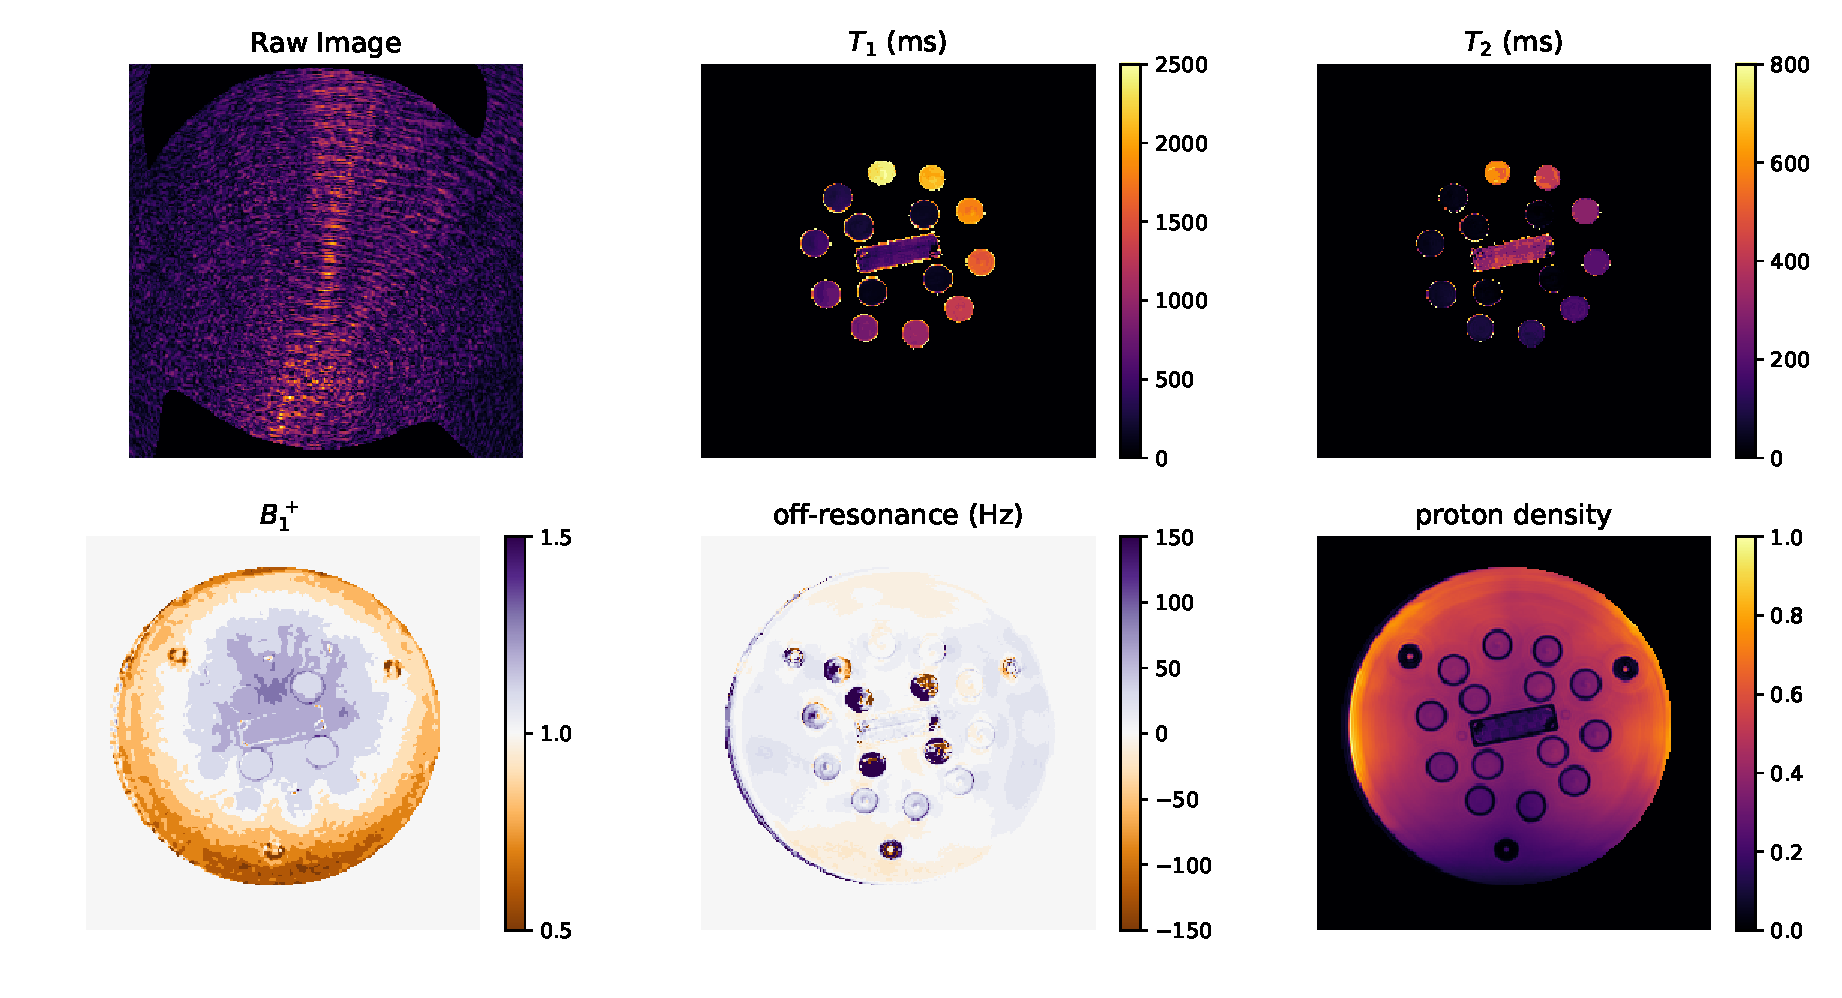
\includegraphics[width=1.2\textwidth]{../img/intro/mrfmap}
	\end{minipage}
\end{frame}

\begin{frame}
	\frametitle{MRF的主要部分和问题:}
	\begin{itemize}
		\item 信号采集:选取合适的MR序列和成像参数,如重复时间($T_\mathrm{R}$)
		\item 字典生成:扩展相图(EPG)模型\textbf{十分耗时且复杂!} $\Rightarrow$ 梯度场、射频场、驰豫等
		\item 匹配算法:模板匹配算法\textbf{十分耗时!} $\Rightarrow$ $O(NL^2K)$
		
		$X=\{x_n\in \mathbb{C}^L, n=1,...,N\}$为指纹数据,$D=\{d_k\in \mathbb{C}^L,k=1,...,K\}$为生成的字典,$L$为时间点的个数。模板匹配算法为:
			\begin{equation*}
	\hat{k}_n = \argmax_k \left|\left\langle d_k,x_n \right\rangle \right|,\quad
	\hat{\rho}_n= \left|\left\langle d_{\hat{k}_n},x_n \right\rangle \right|
	\end{equation*}
	\end{itemize}
	
%	模板匹配的运行时间与字典大小$K$,时间点的个数$L$以及指纹数据中体素的个数有关,计算复杂度为$O(NL^2K)$
\end{frame}


%\begin{frame}
%\frametitle{研究背景--MRF}
%	MRF重建的主要问题:
%	\begin{itemize}
%		\item 字典生成和模板匹配的速度慢,当字典比较大时,通常需要几十分钟甚至几小时。
%		\item 临床中还无法应用,需要快速甚至实时的算法
%	\end{itemize}
%\end{frame}

\subsection{CUDA程序实现}
\begin{frame}
	\frametitle{图形处理单元(GPU)}
	\begin{itemize}
		\item 图形处理单元(GPU)逐渐成为并行加速科学计算的主流方法,在医学成像领域有着广泛的应用	
		\item GPU中集成了大规模并行计算单元,用于浮点运算
		\item CUDA是NVIDIA公司的应用程序接口,为用户提供了可编程的特性
		\item \textbf{首次}在CUDA的框架下,利用GPU来实现并行加速MRF字典生成与模板匹配,并设计开发了一款开源程序snapMRF
	\end{itemize}

\end{frame}

\begin{frame}
	\frametitle{snapMRF程序流程}
%	\begin{figure}
%\begin{minipage}[t]{0.5\textwidth}
%\includegraphics[width=0.5\textwidth]{../img/snapmrf/snapMRF.png}
%\end{minipage}
%\begin{center}
	\scalebox{0.55}{
	\begin{minipage}{0.5\linewidth}
	\includegraphics[width=1\textwidth]{../img/snapmrf/snapMRF.png}
	\end{minipage}
	\hspace{1.5cm}
	\begin{minipage}{1.2\linewidth}
	\begin{algorithm}[H]
	\caption{snapMRF生成字典与模板匹配详细流程}
	\label{alg:snapMRF}
	\begin{algorithmic}
		\INDSTATE[-1] \textbf{输入:}\texttt{*d\_mrf},\texttt{*d\_params},\texttt{*d\_img}
		\INDSTATE[-1] \textbf{输出:}\texttt{*d\_atoms},\texttt{*d\_maps}
		\STATE 01:从CSV文件中读取MRF序列信息,存入\texttt{*d\_mrf};
		\STATE 02:从命令行输入字典参数信息,存入\texttt{*d\_params};
		\STATE 03:初始化状态矩阵\texttt{*d\_w};
		\STATE 04:\textbf{迭代}:从第1个时刻到第$L$个时刻,并行计算字典中所有元素
		\STATE 05:\qquad 使用函数\texttt{fill\_transition\_matrix()}构造转移矩阵;
		\STATE 06:\qquad 使用函数\texttt{apply\_rf\_pulse()}将射频场作用在\texttt{*d\_w}上;
		\STATE 07:\qquad 使用函数\texttt{decay\_signal()}将$T_1$和$T_2$衰减作用在\texttt{*d\_w}上;
		\STATE 08:\qquad 使用函数\texttt{save\_atoms()}将元素的信号保存在\texttt{*d\_atoms}中;
		\STATE 09:\qquad 使用函数\texttt{dephase\_gradients()}将梯度场作用在\texttt{*d\_w}上;
		\STATE 10:\qquad 使用函数\texttt{decay\_signal()}将$T_1$和$T_2$衰减作用在\texttt{*d\_w}上;
		\STATE 11:\textbf{终止迭代};
		\STATE 12:释放\texttt{*d\_w};
		\STATE 13:从RawArray文件中读取指纹数据,存入\texttt{*d\_img};
		\STATE 14:计算剩余显存大小,并根据剩余显存,将\texttt{*d\_img}分为$G$组;
		\STATE 15:\textbf{迭代}:从第1组到第$G$组,在每一组内并行计算所有体素的参数
		\STATE 16:\qquad 使用函数\texttt{MRF\_minimatch()}进行匹配;
		\STATE 17:\qquad 使用函数\texttt{generate\_maps()}生成参数图;
		\STATE 18:\textbf{终止迭代};
		\STATE 19:将\texttt{*d\_atoms}和\texttt{*d\_maps}保存为RawArray文件;
		\STATE 20:释放所有显存和内存。
	\end{algorithmic}
\end{algorithm}
\end{minipage}}
%\end{center}
%\hspace{2cm}
%\begin{minipage}{0.5\linewidth}
%	\includegraphics[width=1\textwidth]{../img/snapmrf/snapMRF.png}
%	\end{minipage}}
\end{frame}

\begin{frame}
	\frametitle{snapMRF的难点与创新}
	\begin{itemize}
		\item 确定一个合适的并行方案
		\item 确定多维向量在显存中的储存结构
		\item 计算多维向量在显存中对应的一维指标
		\item 将EPG算法生成字典的过程分裂为小的GPU核函数
		\item 管理显存
		\item 避免数据在GPU与CPU之间多次拷贝
	\end{itemize}
\end{frame}

%------------------------------------------------
\subsection{数值实验结果与分析}
\begin{frame}
	\frametitle{数值实验结果}
		\begin{figure}[htbp]
\begin{minipage}[t]{0.45\textwidth}
\centering
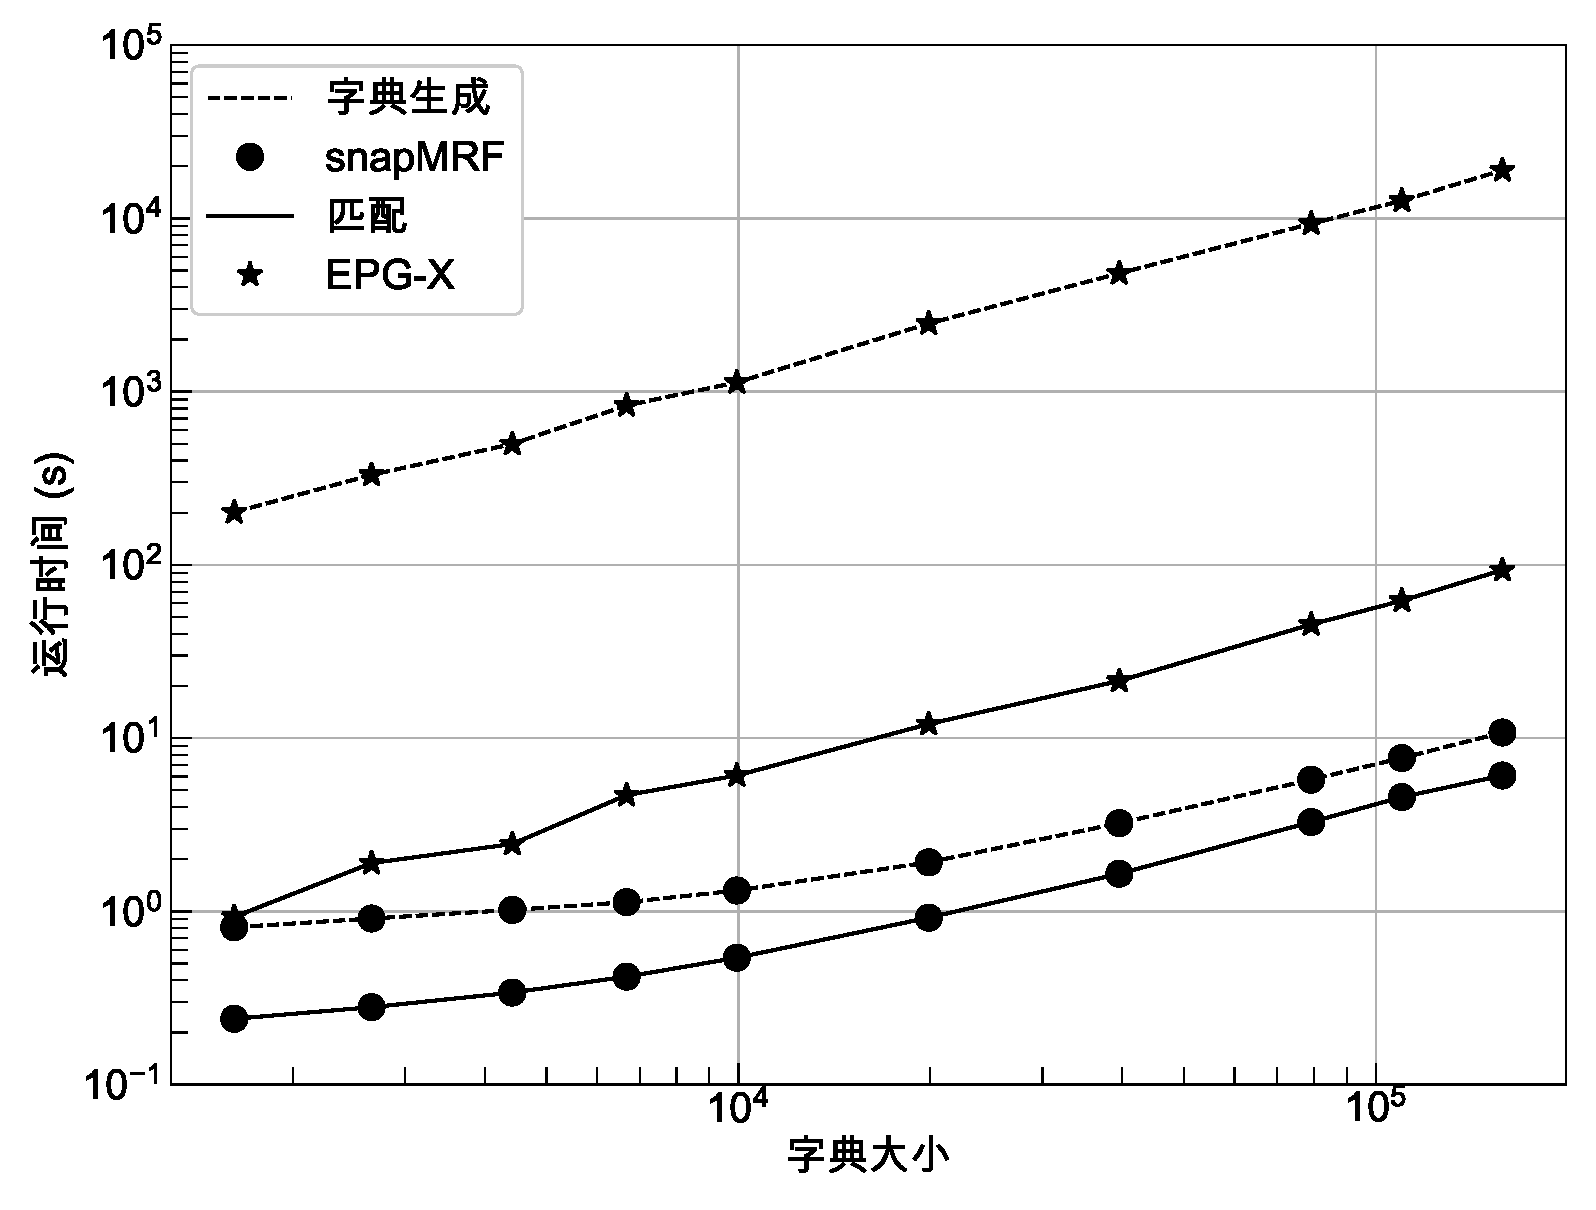
\includegraphics[width=1.1\textwidth]{../img/snapmrf/time_vs_epgx.eps}
\\ snapMRF vs EPG-X
\end{minipage}
\hspace{0.5cm}
\begin{minipage}[t]{0.45\textwidth}
\centering
\includegraphics[width=1.1\textwidth]{../img/snapmrf/time_vs_pnp.eps}
\\ snapMRF vs PnP-MRF
\end{minipage}
\end{figure}
\end{frame}


\begin{frame}
%\frametitle{实验结果}
\begin{table}
\caption{snapMRF与EPG-X在字典生成和模板匹配上运行时间的比较}
\centering
\label{tab:time}
\begin{tabular}{|l|l|l|l|l|l|}
\hline
\hline
运行时间 & EPG-X & snapMRF & snapMRF & snapMRF\\ 
(s) & 固定$T_\mathrm{R}$ & 固定$T_\mathrm{R}$ & 变化$T_\mathrm{R}$ & 变化$T_\mathrm{R}$+$B_1^+$\\
\hline
体模/字典生成 & 17797.05 & 11.00 & 7.42 & 9.39 \\
\hline
体模/模板匹配 & 137.13 & 5.97 & 4.14 & 4.88\\
\hline
脑部/字典生成 & 18629.82 & 11.29 & 7.63 & 8.72 \\
\hline
脑部/模板匹配 & 143.55 & 6.13 & 4.23 & 4.63 \\
\hline
\end{tabular}
\end{table}
\begin{itemize}
	\item 字典大小$1,000\times 100,000$
	\item 指纹大小$1,000\times 240\times 240$
\end{itemize}
\end{frame}

\begin{frame}
\scalebox{0.6}{
	\hspace{-1.8cm}
	\begin{minipage}[t]{1\linewidth}
	\begin{table}
	\caption{$T_1$参数图的准确性比较}
\centering
\label{tab:t1}
\begin{tabular}{|l|l|l|l|l|l|}
\hline
\hline
真实$T_1$ & EPG-X & snapMRF & snapMRF & snapMRF\\ 
(ms) & 固定$T_\mathrm{R}$ & 固定$T_\mathrm{R}$ & 变化$T_\mathrm{R}$ & 变化$T_\mathrm{R}$+$B_1^+$\\
\hline
90.9 & 128.5 & 127.7 & 111.5 & 94.2\\
\hline
126.9 & 155.0 & 155.0 & 146.5 & 127.9\\
\hline
176.6 & 173.1 & 173.1 & 172.3 & 153.8\\
\hline
244.2 & 280.4 & 280.4 & 265.0 & 225.0\\
\hline
336.5 & 342.7 & 342.7 & 326.5 & 319.2\\
\hline
458.4 & 471.2 & 471.2 & 471.9 & 468.3\\
\hline
608.6 & 602.7 & 601.2 & 625.0 & 622.1\\
\hline
801.7 & 771.5 & 770.4 & 818.5 & 813.5\\
\hline
1044.0 & 945.0 & 943.1 & 1032.3 & 1026.0\\
\hline
1332.0 & 1262.7 & 1263.1 & 1310.8 & 1306.7\\
\hline
1604.0 & 1568.8 & 1568.1 & 1607.3 & 1593.3\\
\hline
1907.0 & 1861.2 & 1861.9 & 1854.2 & 1828.8\\
\hline
2173.0 & 2043.1 & 2043.1 & 2091.9 & 2094.2\\
\hline
2480.0 & 2366.5 & 2366.2 & 2434.6 & 2416.3\\
\hline
err (\%) & 4.9 & 5.0 & 2.6 & 3.0\\
 
\hline
\end{tabular}
\end{table}
\end{minipage}
\hspace{-0.4cm}
	\begin{minipage}[t]{1\linewidth}
	\begin{table}
\caption{$T_2$参数图的准确性比较}
\centering
\label{tab:t2}
\begin{tabular}{|l|l|l|l|l|l|}
\hline
\hline
真实$T_2$ & EPG-X & snapMRF & snapMRF & snapMRF\\ 
(ms) & 固定$T_\mathrm{R}$ & 固定$T_\mathrm{R}$ & 变化$T_\mathrm{R}$ & 变化$T_\mathrm{R}$+$B_1^+$\\
\hline
5.6 & 6.9 & 6.9 & 9.4 & 12.3\\
\hline
7.9 & 11.5 & 11.2 & 10.0 & 13.5\\
\hline
11.2 & 13.3 & 13.3 & 11.2 & 13.5\\
\hline
15.8 & 13.7 & 13.5 & 11.3 & 20.4\\
\hline
22.6 & 21.2 & 21.2 & 23.3 & 30.0\\
\hline
32.0 & 32.3 & 32.3 & 38.3 & 47.3\\
\hline
46.4 & 45.0 & 44.8 & 50.4 & 60.0\\
\hline
64.1 & 64.2 & 64.2 & 70.2 & 83.8\\
\hline
96.9 & 84.6 & 84.4 & 90.8 & 104.6\\
\hline
133.3 & 144.0 & 143.8 & 146.9 & 170.8\\
\hline
190.9 & 175.4 & 175.4 & 185.2 & 213.8\\
\hline
278.1 & 266.5 & 266.5 & 255.4 & 290.0\\
\hline
403.5 & 323.3 & 323.5 & 343.7 & 407.7\\
\hline
581.3 & 474.0 & 474.2 & 453.5 & 531.5\\
\hline
err (\%) & 16.9 & 16.9 & 17.9 & 9.3\\

\hline
\end{tabular}
\end{table}
	\end{minipage}
}

\end{frame}

\begin{frame}
%\frametitle{实验结果}
\begin{figure}
\centering
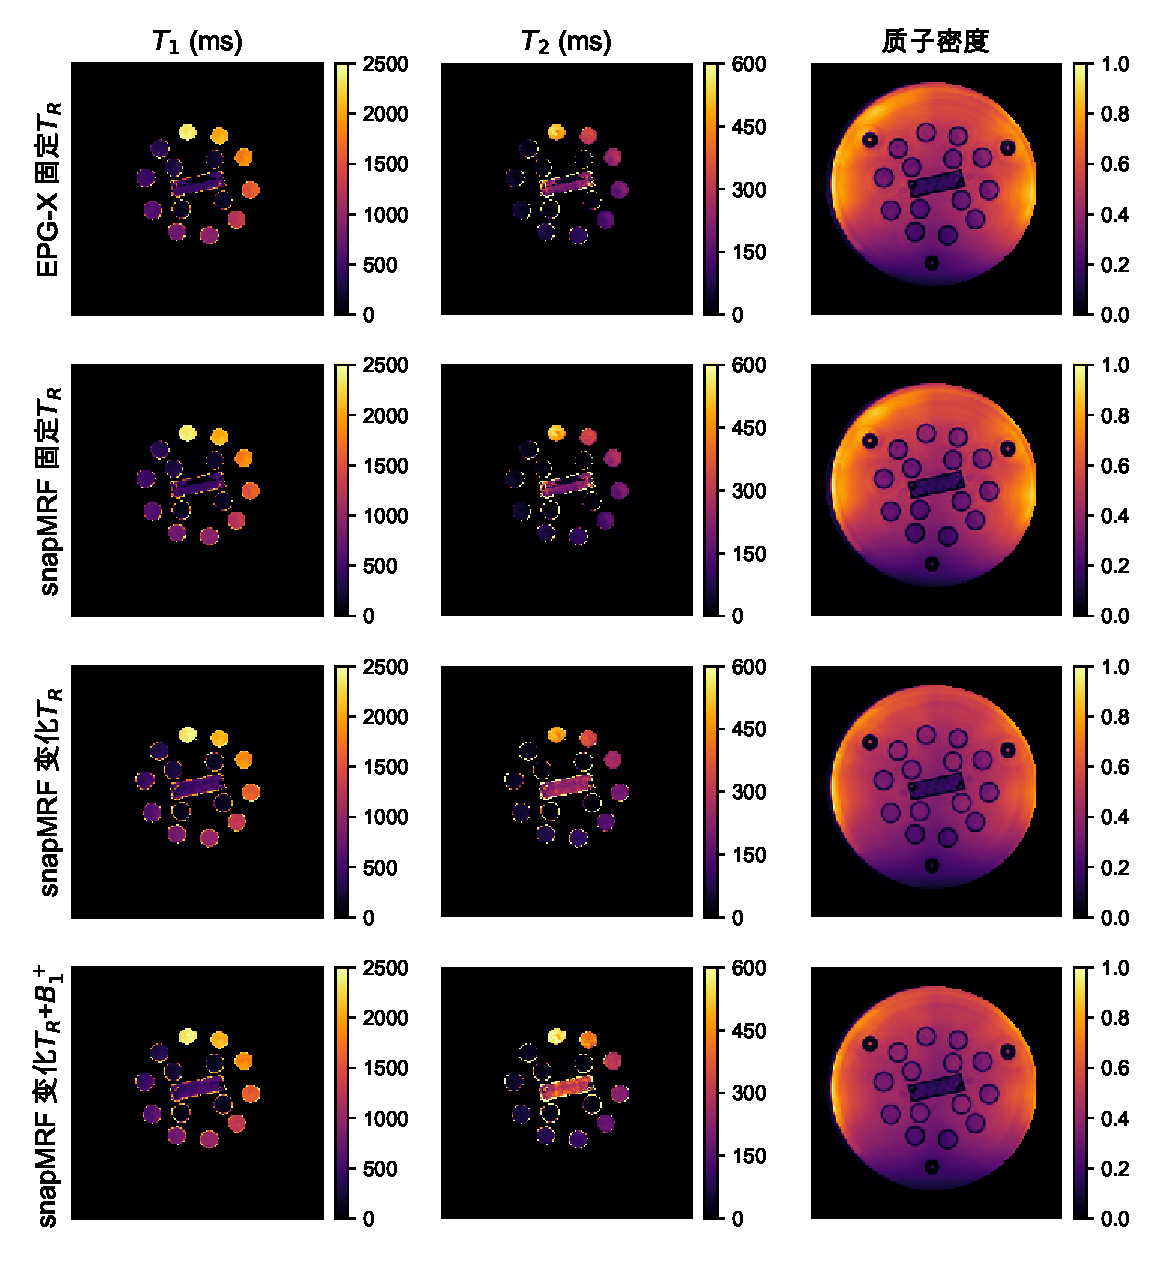
\includegraphics[width=0.65\textwidth]{../img/snapmrf/figure2.eps}
\end{figure}
\end{frame}

\begin{frame}
%\frametitle{实验结果}
\begin{figure}
\centering
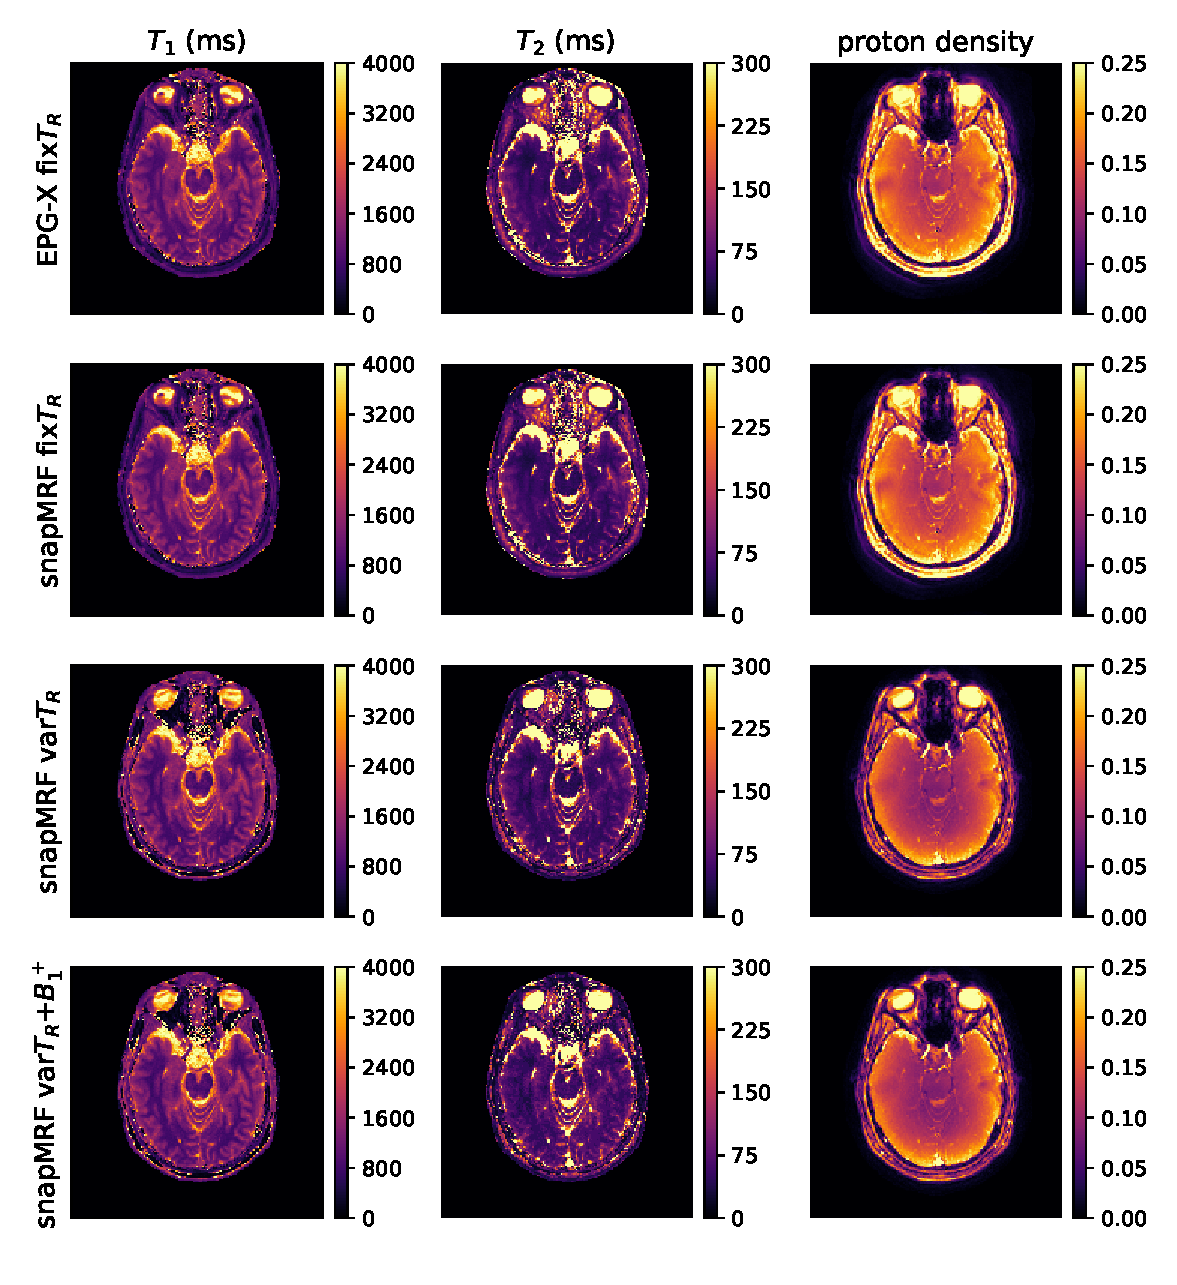
\includegraphics[width=0.65\textwidth]{../img/snapmrf/figure3.eps}
\end{figure}
\end{frame}

%------------------------------------------------
\section{全文总结}

\begin{frame}
    \tableofcontents[currentsection,hideallsubsections]
\end{frame}

\begin{frame}
	\textbf{本文工作:}
	\begin{itemize}
		\item 提出了动态MR图像的重建模型$\Rightarrow$ \textbf{二阶时空TGV+核范数},优于其他的重建模型,尤其是在胸部DCE-MRI图像上
		\item \textbf{首次}从定量分析的角度评估胸部DCE-MRI图像的时间方向的稀疏正则项$\Rightarrow$ TV/TGV可以得到最准确的定量参数,核范数可以提高重建图像的整体信噪比
		\item \textbf{首次}在CUDA框架下进行MRF字典生成和匹配$\Rightarrow$ snapMRF字典生成的速度提高了10--1000$\times$,模板匹配的速度提高了10--100$\times$,并在多种MR序列中都可以生成高质量的参数图。
	\end{itemize}
	
	\textbf{未来考虑:}
	\begin{itemize}
		\item 其他类型的医学成像:CT、US等
		\item 变分模型+深度神经网络:将变分模型按迭代算法展开成一个深度神经网络
	\end{itemize}
\end{frame}


%------------------------------------------------

\begin{frame}
\centerline{感谢各位专家、老师来参加我的博士论文学位答辩!}
\end{frame}

%----------------------------------------------------------------------------------------
\end{document}